%%% Original version by Donald Craig.
%%% Modified by Theodore Norvell 2009 November 25


\documentclass[12pt]{report}
%%%%%%%%%%%%%%%%%%%%%%%%%%%%%%%%%%%%%%%%%%%%%%%%%%%%%%%%%%%%%%%%%%%%%%%%%%%%%%%%%%%%%%%%%%%%%%%%%%%%%%%%%%%%%%%%%%%%%%%%%%%%%%%%%%%%%%%%%%%%%%%%%%%%%%%%%%%%%%%%%%%%%%%%%%%%%%%%%%%%%%%%%%%%%%%%%%%%%%%%%%%%%%%%%%%%%%%%%%%%%%%%%%%%%%%%%%%%%%%%%%%%%%%%%%%%
\usepackage{makeidx}
\usepackage{eurosym}
\usepackage{mun-thesis}
\usepackage{amsmath}
\usepackage{amsfonts}
\usepackage{amssymb}
\usepackage{graphicx}
\usepackage{float}
\usepackage{code}
\usepackage{listings}
\usepackage{comment}
\usepackage{thesis.zeros}
\usepackage{accents}
\usepackage{named.cite}
\usepackage{hyperref}

\setcounter{MaxMatrixCols}{10}
%TCIDATA{OutputFilter=LATEX.DLL}
%TCIDATA{Version=5.50.0.2960}
%TCIDATA{<META NAME="SaveForMode" CONTENT="3">}
%TCIDATA{BibliographyScheme=BibTeX}
%TCIDATA{Created=Thursday, October 21, 2010 17:39:22}
%TCIDATA{LastRevised=Thursday, December 17, 2015 13:41:42}
%TCIDATA{<META NAME="GraphicsSave" CONTENT="32">}
%TCIDATA{<META NAME="DocumentShell" CONTENT="Theses\MUN Thesis">}
%TCIDATA{CSTFile=mun-thesis.cst}

\renewcommand{\theequation}{\thechapter.\fromz{equation}}
\lstset{ 
        columns=fullflexible,
        tabsize=4,showtabs=false,
        showspaces=false,
        showstringspaces=true,
        numbers=left, stepnumber=5, firstnumber=0,
         captionpos=b,
         breaklines=true,
         postbreak={\raisebox{0ex}[0ex][0ex]{\ensuremath{\hookrightarrow}}},
         prebreak={\raisebox{0ex}[0ex][0ex]{\ensuremath{\hookleftarrow}}},
         breakautoindent=false,
         breakindent=0pt,
         keywordstyle=\bfseries,
         identifierstyle=\sffamily,
         commentstyle=\itshape,
         stringstyle=\ttfamily}
\lstnewenvironment{lstfloatinglisting}{\lstset{float=tb}}{}
\renewcommand{\lstlistlistingname}{List of Listings}
\AtBeginDocument{\renewcommand\thelstlisting{\thechapter.\fromz{lstlisting}}}
\floatstyle{plain}
\floatname{algorithm}{Algorithm}
\newfloat{algorithm}{tb}{loa}[chapter]
\renewcommand{\thealgorithm}{\thechapter.\fromz{algorithm}}
\newtheorem{theorem}{Theorem}[chapter]
\newtheorem{axiom}[theorem]{Axiom}
\newtheorem{claim}[theorem]{Claim}
\newtheorem{conclusion}[theorem]{Conclusion}
\newtheorem{condition}[theorem]{Condition}
\newtheorem{conjecture}[theorem]{Conjecture}
\newtheorem{corollary}[theorem]{Corollary}
\newtheorem{criterion}[theorem]{Criterion}
\newtheorem{definition}[theorem]{Definition}
\newtheorem{example}[theorem]{Example}
\newtheorem{exercise}[theorem]{Exercise}
\newtheorem{lemma}[theorem]{Lemma}
\newtheorem{notation}[theorem]{Notation}
\newtheorem{problem}[theorem]{Problem}
\newtheorem{proposition}[theorem]{Proposition}
\newtheorem{remark}[theorem]{Remark}
\newtheorem{solution}[theorem]{Solution}
\newtheorem{summary}[theorem]{Summary}
\input{tcilatex}
\begin{document}


%TCIMACRO{\QSubDoc{Include frontMatter}{%TCIDATA{Version=5.50.0.2960}
%TCIDATA{LaTeXparent=0,0,Master.tex}
                      

\pagenumbering{roman}%
%TCIMACRO{\TeXButton{Start at page 0}{\addtocounter{page}{-1}}}%
%BeginExpansion
\addtocounter{page}{-1}%
%EndExpansion

\begin{comment}
To edit the title page, double click on the grey Title\ Page box below.
\end{comment}

%TCIMACRO{%
%\TeXButton{Title Page}{\thesistitle
%{Meta-thesis for Scientific Word:\\How to Use \LaTeX
%\ to Typeset Your MUN Thesis}{Theodore S.~Norvell}{Master of Engineering (Computer Engineering)}{Faculty of Engineering and Applied Science}{December 2012}}}%
%BeginExpansion
\thesistitle
{Meta-thesis for Scientific Word:\\How to Use \LaTeX
\ to Typeset Your MUN Thesis}{Theodore S.~Norvell}{Master of Engineering (Computer Engineering)}{Faculty of Engineering and Applied Science}{December 2012}%
%EndExpansion

\newpage\renewcommand{\baselinestretch}{\double}%
\addcontentsline{toc}{chapter}{Abstract}

\begin{center}
\textbf{\large Abstract}
\end{center}

This document provides information on how to write your thesis using the %
\LaTeX\ document preparation system. You can use the files used to generate
this paper as a template for your own thesis.

You should put your real abstract here, of course.

\newpage\addcontentsline{toc}{chapter}{Acknowledgements}

\begin{center}
\textbf{\large Acknowledgements}
\end{center}

Based on Meta-Thesis by Donald Craig. Philip Viton helped with the listings
package. Of course thanks are due to everyone at MacKichen software, Donald
Knuth, Leslie Lamport, and the many other developers who have made this all
possible.

\renewcommand{\baselinestretch}{\single}

%TCIMACRO{\TeXButton{Table of Contents}{\tableofcontents}}%
%BeginExpansion
\tableofcontents%
%EndExpansion

%TCIMACRO{%
%\TeXButton{List of Tables}{\addcontentsline{toc}{chapter}{List of Tables}
%\listof{table}{List of Tables}}}%
%BeginExpansion
\addcontentsline{toc}{chapter}{List of Tables}
\listof{table}{List of Tables}%
%EndExpansion

%TCIMACRO{%
%\TeXButton{List of Figures}{\addcontentsline{toc}{chapter}{List of Figures}
%\listof{figure}{List of Figures}}}%
%BeginExpansion
\addcontentsline{toc}{chapter}{List of Figures}
\listof{figure}{List of Figures}%
%EndExpansion

%TCIMACRO{%
%\TeXButton{List of Listings}{\addcontentsline{toc}{chapter}{List of Listings}
%\lstlistoflistings}}%
%BeginExpansion
\addcontentsline{toc}{chapter}{List of Listings}
\lstlistoflistings%
%EndExpansion

%TCIMACRO{%
%\TeXButton{List of Algorithms}{\addcontentsline{toc}{chapter}{List of Algorithms}
%\listof{algorithm}{List of Algorithms}}}%
%BeginExpansion
\addcontentsline{toc}{chapter}{List of Algorithms}
\listof{algorithm}{List of Algorithms}%
%EndExpansion

%TCIMACRO{%
%\TeXButton{List of Abbreviations}{\addcontentsline{toc}{chapter}{List of Abbreviations}
%\chapter*{List of Abbreviations}}}%
%BeginExpansion
\addcontentsline{toc}{chapter}{List of Abbreviations}
\chapter*{List of Abbreviations}%
%EndExpansion
\begin{tabular}[t]{lll}
GNU & \qquad \qquad & GNU's not UNIX \\ 
LOA &  & List of Abbreviations \\ 
TLA &  & Three Letter Acronym \\ 
&  &  \\ 
&  & 
\end{tabular}

%TCIMACRO{%
%\TeXButton{List of Notations}{\addcontentsline{toc}{chapter}{List of Notations}
%\chapter*{List of Notations}}}%
%BeginExpansion
\addcontentsline{toc}{chapter}{List of Notations}
\chapter*{List of Notations}%
%EndExpansion
\begin{tabular}[t]{lll}
$f:a\rightarrow b$ & \qquad \qquad & $f$ is an arrow from $a$ to $b$ \\ 
$\overrightarrow{f}$ &  & The target of $f$ \\ 
$\overleftarrow{f}$ &  & The source of $f$ \\ 
$\limfunc{id}(a)$ &  & The identity arrow of $f$ \\ 
$f;g$ &  & The composition of $f$ and $g$ where $\overrightarrow{f}=%
\overleftarrow{g}$%
\end{tabular}
}}%
%BeginExpansion
%TCIDATA{Version=5.50.0.2960}
%TCIDATA{LaTeXparent=0,0,Master.tex}
                      

\pagenumbering{roman}%
%TCIMACRO{\TeXButton{Start at page 0}{\addtocounter{page}{-1}}}%
%BeginExpansion
\addtocounter{page}{-1}%
%EndExpansion

\begin{comment}
To edit the title page, double click on the grey Title\ Page box below.
\end{comment}

%TCIMACRO{%
%\TeXButton{Title Page}{\thesistitle
%{Meta-thesis for Scientific Word:\\How to Use \LaTeX
%\ to Typeset Your MUN Thesis}{Theodore S.~Norvell}{Master of Engineering (Computer Engineering)}{Faculty of Engineering and Applied Science}{December 2012}}}%
%BeginExpansion
\thesistitle
{Meta-thesis for Scientific Word:\\How to Use \LaTeX
\ to Typeset Your MUN Thesis}{Theodore S.~Norvell}{Master of Engineering (Computer Engineering)}{Faculty of Engineering and Applied Science}{December 2012}%
%EndExpansion

\newpage\renewcommand{\baselinestretch}{\double}%
\addcontentsline{toc}{chapter}{Abstract}

\begin{center}
\textbf{\large Abstract}
\end{center}

This document provides information on how to write your thesis using the %
\LaTeX\ document preparation system. You can use the files used to generate
this paper as a template for your own thesis.

You should put your real abstract here, of course.

\newpage\addcontentsline{toc}{chapter}{Acknowledgements}

\begin{center}
\textbf{\large Acknowledgements}
\end{center}

Based on Meta-Thesis by Donald Craig. Philip Viton helped with the listings
package. Of course thanks are due to everyone at MacKichen software, Donald
Knuth, Leslie Lamport, and the many other developers who have made this all
possible.

\renewcommand{\baselinestretch}{\single}

%TCIMACRO{\TeXButton{Table of Contents}{\tableofcontents}}%
%BeginExpansion
\tableofcontents%
%EndExpansion

%TCIMACRO{%
%\TeXButton{List of Tables}{\addcontentsline{toc}{chapter}{List of Tables}
%\listof{table}{List of Tables}}}%
%BeginExpansion
\addcontentsline{toc}{chapter}{List of Tables}
\listof{table}{List of Tables}%
%EndExpansion

%TCIMACRO{%
%\TeXButton{List of Figures}{\addcontentsline{toc}{chapter}{List of Figures}
%\listof{figure}{List of Figures}}}%
%BeginExpansion
\addcontentsline{toc}{chapter}{List of Figures}
\listof{figure}{List of Figures}%
%EndExpansion

%TCIMACRO{%
%\TeXButton{List of Listings}{\addcontentsline{toc}{chapter}{List of Listings}
%\lstlistoflistings}}%
%BeginExpansion
\addcontentsline{toc}{chapter}{List of Listings}
\lstlistoflistings%
%EndExpansion

%TCIMACRO{%
%\TeXButton{List of Algorithms}{\addcontentsline{toc}{chapter}{List of Algorithms}
%\listof{algorithm}{List of Algorithms}}}%
%BeginExpansion
\addcontentsline{toc}{chapter}{List of Algorithms}
\listof{algorithm}{List of Algorithms}%
%EndExpansion

%TCIMACRO{%
%\TeXButton{List of Abbreviations}{\addcontentsline{toc}{chapter}{List of Abbreviations}
%\chapter*{List of Abbreviations}}}%
%BeginExpansion
\addcontentsline{toc}{chapter}{List of Abbreviations}
\chapter*{List of Abbreviations}%
%EndExpansion
\begin{tabular}[t]{lll}
GNU & \qquad \qquad & GNU's not UNIX \\ 
LOA &  & List of Abbreviations \\ 
TLA &  & Three Letter Acronym \\ 
&  &  \\ 
&  & 
\end{tabular}

%TCIMACRO{%
%\TeXButton{List of Notations}{\addcontentsline{toc}{chapter}{List of Notations}
%\chapter*{List of Notations}}}%
%BeginExpansion
\addcontentsline{toc}{chapter}{List of Notations}
\chapter*{List of Notations}%
%EndExpansion
\begin{tabular}[t]{lll}
$f:a\rightarrow b$ & \qquad \qquad & $f$ is an arrow from $a$ to $b$ \\ 
$\overrightarrow{f}$ &  & The target of $f$ \\ 
$\overleftarrow{f}$ &  & The source of $f$ \\ 
$\limfunc{id}(a)$ &  & The identity arrow of $f$ \\ 
$f;g$ &  & The composition of $f$ and $g$ where $\overrightarrow{f}=%
\overleftarrow{g}$%
\end{tabular}
%
%EndExpansion

\begin{comment}
Remember to save all subdocuments before typesetting.
\end{comment}

\renewcommand{\baselinestretch}{\double}

%TCIMACRO{\QSubDoc{Include chIntro}{%TCIDATA{Version=5.50.0.2960}
%TCIDATA{LaTeXparent=0,0,Master.tex}
                      
%TCIDATA{ChildDefaults=chapter:1,page:1}


\chapter{Introduction}

\label{chap:intro}

\begin{comment}
The two TeX boxes on the following line should only be used for the first
chapter
\end{comment}

%TCIMACRO{\TeXButton{pagenumbering}{\pagenumbering{arabic}}}%
%BeginExpansion
\pagenumbering{arabic}%
%EndExpansion
%TCIMACRO{\TeXButton{Start at page 0}{\addtocounter{page}{-1}}}%
%BeginExpansion
\addtocounter{page}{-1}%
%EndExpansion

\begin{quotation}
\LaTeX is a system for typesetting documents. Its first widely available
version, mysteriously numbered 2.09, appeared in 1985. \LaTeX{} is now
extremely popular in the scientific and academic communities, and it is used
extensively in industry. It has become a \emph{lingua franca} of the
scientific world; scientists send their papers electronically to colleagues
around the world in the form of \LaTeX{} input.\cite{Lamport-1994}
\end{quotation}

\section{Getting started}

This document serves three purposes.

\begin{itemize}
\item It contains some information on how to use \LaTeX~\cite{Lamport-1994}
and Scientific Word to typeset your thesis.

\item It serves as a template that you can use for your thesis. Make a copy.

\item It contains many examples and some advice.
\end{itemize}

By default, all text is double spaced, however, lengthy quotations and
footnotes must be singled spaced. The left margin is slightly wider than the
right margin. This is to compensate for binding.

See \url{http://www.mun.ca/sgs/go/guid_policies/guidelines_intro.php} for
the SGS\ guidelines.

\section{Some tips, pitfalls, and opinions}

\label{sec:hints}

\subsection{Text mode}

\begin{itemize}
\item Use the View menu to turn on all the following:\ Invisibles, Helper
lines, Helper Boxes, Markers, Status Bar. Use View\ \TEXTsymbol{>}%
\TEXTsymbol{>}\ Toolbars to ensure that most tool bars are displayed. (I\
use all except History and Exam). Rearrange the tool bars with the mouse
until you are happy.

\item In text mode, type ` twice to get a \textquotedblleft\ and type '
twice to get \textquotedblright .

\item In LaTeX a closing single quotation mark and an apostrophe are the
same character. Use the ' key.

\item When you need three `s or three 's in a row, you can use a
\textquotedblleft zero space\textquotedblright\ (see below) to clarify what
is what. For example:\ John said, \textquotedblleft I heard her yell
`Stop'{}\textquotedblright . There is a zero space between the ' and the
\textquotedblright .

\item In text mode, type - twice to get and en-dash --. Type - three times
to get an em-dash --- . (Use en-dashes only for ranges of numbers or years.
Use em-dashes for punctuation.)

\item In text mode, the - key gives a hyphen, not a minus sign. Compare $x-y$
to \textit{x-y}.

\item For various kinds of horizontal spaces Insert \TEXTsymbol{>}%
\TEXTsymbol{>}\ Spacing \TEXTsymbol{>}\TEXTsymbol{>}\ Horizontal space (or
Alt i s h). See table \ref{tab-spaces} for more shortcuts and descriptions.

%TCIMACRO{\TeXButton{B}{\begin{table}[tbp] \centering}}%
%BeginExpansion
\begin{table}[tbp] \centering%
%EndExpansion
%TCIMACRO{\TeXButton{B SingleSpaced}{\begin{singlespaced}}}%
%BeginExpansion
\begin{singlespaced}%
%EndExpansion
$%
\begin{tabular}{|l|l|l|p{5cm}|}
\hline\hline
\multicolumn{1}{||l|}{\textbf{Space}} &  & \textbf{Shortcut} & 
\multicolumn{1}{|p{5cm}||}{\textbf{Use}} \\ \hline\hline
Normal & a b & Space bar & Text mode \\ \hline
Required & etc.\ a & Shift-space\  & Text mode, after a ., !, or ? that does
not end a sentence \\ \hline
Nonbreaking & Table~\ref{tab-spaces} & Cntl-space & Text mode, where a line
break would be confusing. \\ \hline
Em-space & a\quad b &  & Math or text mode. \\ \hline
2 em-space & a\qquad b &  & Math or text mode. \\ \hline
Thin space & $x\,y$ & Cntl-, & In math mode only. \\ \hline
Thick space & $x\;y$ & Cntl-Shift-space & In math mode only. \\ \hline
Italic correction & \textit{f}\/; &  & If needed, between italic and roman
characters. \\ \hline
Zero space & '{}\textquotedblright &  & Between ' and \textquotedblright\ or
` and \textquotedblleft . \\ \hline
Negative thin & $\cap \!\!\!\bullet $ &  & Math only. (Best to avoid the
need.) \\ \hline
No indent &  &  & Before a paragraph that should not be indented. \\ \hline
Custom &  &  & When long or stretchy spaces are needed. \\ \hline
\end{tabular}%
$%
%TCIMACRO{\TeXButton{E SingleSpaced}{\end{singlespaced}}}%
%BeginExpansion
\end{singlespaced}%
%EndExpansion
\caption{Horizontal spaces}\label{tab-spaces}%
%TCIMACRO{\TeXButton{E}{\end{table}}}%
%BeginExpansion
\end{table}%
%EndExpansion

\item You can double click on a space to change its width and nature. I\
find it easier to select the space and hit Control-F5

\item Tip:\ You can change the properties of spaces, letters, tables, and
other objects by selecting the object and hitting Control-F5.

\item Pitfall:\ Speaking of spaces. LaTeX will insert a little an
extra-stretchy space between sentences. About 99\% of the time\ LaTeX has no
problem correctly identifying the end of a sentence. The rule is this:\ Any
period (.), exclamation point (!), or question mark (?) that does not follow
a capital letter and that is followed by a normal space marks the end of a
sentence. So:

\begin{itemize}
\item When a period (.), exclamation point (!), or question mark (?) does
not end a sentence, follow it with a \textquotedblleft nonbreaking
space\textquotedblright\ (Alt i s h b) or a \textquotedblleft required
space\textquotedblright\ (Alt i s h r). For example, if I\ wrote
\textquotedblleft Dr.~N. loves C%
%TCIMACRO{\TeXButton{@}{\@}}%
%BeginExpansion
\@%
%EndExpansion
.\textquotedblright , I'd put a nonbreaking space between \textquotedblleft
Dr.\textquotedblright\ and \textquotedblleft N\textquotedblright . I could
have put a required space between the \textquotedblleft
N.\textquotedblright\ and \textquotedblleft loves\textquotedblright , but
there is no need, as LaTeX will assume that this period does not end a
sentence. I\ chose a nonbreaking space between \textquotedblleft
Dr.\textquotedblright\ and \textquotedblleft N.\textquotedblright\ because I
didn't want a line-break between them. For long surnames, it may be
preferable to use a required space after an abbreviated title.

\item When a period (.), exclamation point (!), or question mark (?) does
end a sentence but also follows a capital letter, put a LaTeX \TEXTsymbol{%
\backslash}@ command between the letter and the punctuation mark. For
example in \textquotedblleft Dr.~N. loves C%
%TCIMACRO{\TeXButton{@}{\@}}%
%BeginExpansion
\@%
%EndExpansion
.\textquotedblright , I'd put a LaTeX \TEXTsymbol{\backslash}@ command
between the \textquotedblleft C\textquotedblright\ and the \textquotedblleft
.\textquotedblright . Alt i y t can be used to insert a TeX command.\ Then
put \TEXTsymbol{\backslash}@ in the text box and click OK.

\item A common error is to put a normal space rather than a required space
after \textquotedblleft i.e.\textquotedblright , \textquotedblleft
e.g.\textquotedblright , \textquotedblleft etc.\textquotedblright\ If they
don't end a sentence, follow it by a required, rather than a normal space.
For example:\ \textquotedblleft CDC, Univac, etc.\ are no more, i.e.\
defunct.\textquotedblright

\item When a period (.), exclamation point (!), or question mark (?) is
followed by a close parenthesis, LaTeX will treat the parenthesis as the end
of the sentence and the following space will be extra stretchy.

\item When a period (.), exclamation point (!), or question mark (?) is
followed by a single or double close quotation mark, LaTeX should treat the
quotation mark as the end of a sentence. However, thanks to an SW oddity,
this won't work with SW. At present I have no good workaround.

\item The following table illustrates how LaTeX deals with various cases:%
%TCIMACRO{\TeXButton{B SingleSpaced}{\begin{singlespaced}}}%
%BeginExpansion
\begin{singlespaced}%
%EndExpansion
\begin{equation*}
\begin{tabular}{|l|p{3.2cm}|}
\hline
Default behaviour & \textquotedblleft (M M m. M MMMM. \\ \hline
Required space & \textquotedblleft (M M m.\ M MMMM. \\ \hline
Paren after period & \textquotedblleft M M m.) M MMMM. \\ \hline
Quote after period. & (M M m.\textquotedblright\ M MMMM. \\ \hline
Period after capital. & \textquotedblleft (m M M. M MMMM. \\ \hline
\TEXTsymbol{\backslash}@ before period & \textquotedblleft (m M M%
%TCIMACRO{\TeXButton{@}{\@}}%
%BeginExpansion
\@%
%EndExpansion
. M MMMM. \\ \hline
\end{tabular}%
\end{equation*}%
%TCIMACRO{\TeXButton{E SingleSpaced}{\end{singlespaced}}}%
%BeginExpansion
\end{singlespaced}%
%EndExpansion
\end{itemize}

\item The `Noindent space' (Insert \TEXTsymbol{>}\TEXTsymbol{>}\ Spacing 
\TEXTsymbol{>}\TEXTsymbol{>}\ Horizontal Space... \TEXTsymbol{>}\TEXTsymbol{>%
}\ Noindent or Alt i s h n) is not really a space at all. It can be used at
the start of a paragraph to suppress its indentation. This is useful when a
list is used that is not at the end of a paragraph.

\item Usually TeX hyphenates without trouble. If it fails to hyphenate \emph{%
Entscheidungsproblem}, for example, correctly you can indicate all the
places where it can hyphenate such troublesome words, using Insert 
\TEXTsymbol{>}\TEXTsymbol{>}\ Spacing \TEXTsymbol{>}\TEXTsymbol{>}\ Break 
\TEXTsymbol{>}\TEXTsymbol{>}\ Discretionany Hyphen.

\item To indicate where line breaks are allowed insert an \textquotedblleft
allow break\textquotedblright\ command (Insert \TEXTsymbol{>}\TEXTsymbol{>}\
Spacing \TEXTsymbol{>}\TEXTsymbol{>}\ Break \TEXTsymbol{>}\TEXTsymbol{>}\
Allow break or Alt i s b a). For example, if I give a file name as
/usr/\allowbreak theo/\allowbreak docs/\allowbreak thesis/\allowbreak
Master.tex. I\ might do well to add an `allow break' after each / except the
first.

\item For URLs and URIs use, Insert \TEXTsymbol{>}\TEXTsymbol{>} TeX Object 
\TEXTsymbol{>}\TEXTsymbol{>} Tex Field ... and insert \texttt{\TEXTsymbol{%
\backslash}url\{\emph{your url}\}}. Follow the link %
\url{http://en.wikibooks.org/wiki/LaTeX/Hyperlinks} for more. This has
several advantages:\ It correctly typesets characters such as tildes. It
allows breaks at the right places. It sets the URL in typewriter font. It
will insert actual hyperlinks into the PDF copy of your thesis, if you
compile it with PDFLaTeX.
\end{itemize}

\subsection{Math mode}

\begin{itemize}
\item Control-m will switch to math mode. Control-t will switch to text mode.

\item I\ set up my User Setup (Tools \TEXTsymbol{>}\TEXTsymbol{>} User
setup) so that the spacebar after a space will switch from text mode to math
mode and a spacebar while in math mode will switch to text mode. That way,
two taps on the spacebar will switch modes and insert a space.

\item To get spaces in math mode, use Control-Shift-Spacebar to get a thick
space $f\;x$ and Control-Comma to get a thin space $f\,x$.

\item In math mode, the - key gives a minus sign, not a hyphen. Compare $x-y$
to \textit{x-y}.

\item In math-mode ' gives you a superscript prime. Compare \textit{x'} to $%
x^{\prime }$. If you really need an apostrophe, closing single quote, or
double quote, switch to text mode.

\item Control-d will insert a new math display as shown in (\ref{eqn:example}%
) 
\begin{equation}
\left( 
\begin{array}{c}
k \\ 
3%
\end{array}%
\right) +\frac{\left( 
\begin{array}{c}
k \\ 
2%
\end{array}%
\right) \left( 
\begin{array}{c}
k-2 \\ 
2%
\end{array}%
\right) }{2}=\frac{1}{(k-2)!}\ \sum_{i=0}^{k-3}(-1)^{i}\left( 
\begin{array}{c}
k-2 \\ 
i%
\end{array}%
\right) (k-2-i)^{k}\text{\quad .}  \label{eqn:example}
\end{equation}

\item When your insertion point (i.e.~caret) is in a math display, the tab
key will toggle whether the display is numbered. Double clicking to the left
or right the display will then bring up a \textquotedblleft display
properties dialog\textquotedblright\ where the \textquotedblleft
key\textquotedblright\ (i.e., \textquotedblleft label\textquotedblright )
can be set. The key is then used in cross references.

\item Multiple line math displays can have separate numbers for each line
and each number is optional. For example%
\begin{eqnarray}
&&\left. f\sqsubseteq g;h\right.   \label{eq:wpreLHS} \\
&=&  \notag \\
&&\left. h\backslash f\sqsubseteq g\right.   \label{eq:wpreRHS}
\end{eqnarray}

\item Opinion:\ Displays should be used when a formula might cause a bad
line break, when the formula is so tall that it will cause an irregular
distance between lines of text, when a formula is long, or when it needs a
number.

\item Opinion: It is good style to only number those displays that need to
be referred to in the text. I.e., that will be cross referenced.

\item Opinion:\ Usually it is best to \textbf{not} omit punctuation after
displayed math. I\ usually leave an em-space or a quad-space between the
math and the punctuation. For example:\ Now it is time to prove%
\begin{equation*}
P\sqsubseteq Q\text{\quad .}
\end{equation*}%
I make an exception\ for computer code. For example:\ 
\begin{equation*}
\text{\texttt{rm -r -f tmp}\quad .}
\end{equation*}%
If the period at the end of that sentence were ,misunderstood to be part of
the code, the meaning of the code would change considerably. The IEEE style
guide suggests omitting the period at the end of sentence, but not other
punctuation.

\item Pitfall: After a display, be careful to only start a new paragraph if
you need one.

\item Pitfall: Multi-character identifiers should not be set in math mode's
default italic font, like this $\sin (first)$. Instead use the \textit{italic%
} font, like this $\sin (\mathit{first})$. The reason is that TeX uses
slightly different fonts for \textquotedblleft math
italic\textquotedblright\ and \textquotedblleft italic\textquotedblright .
The math italic font is designed so that the spacing between adjacent
letters is correct for implicit multiplication or function application $xy+fx
$. The italic font is designed so the letter spacing is correct for words.
(I\ have set Shift-F6 to give \textit{italic font}.)

\item Opinion:\ I\ generally use italic (or math italic, if only one letter
is used)\ for variables and \textrm{an upright font such as Roman}
(Shift-F4) or \textsf{sans-serif} (Shift-F5) for constants, e.g. $\sin (x)$,
but $f(\mathrm{e})$. However, as Alan Perlis once said, \textquotedblleft
one man's constant is another man's variable\textquotedblright . If a
certain sequence of letters is intended to represent exactly the same thing
everywhere in your thesis, it's probably a constant. Otherwise, it is
probably a variable. (Aside:\ Strictly speaking, the opinion that constants
should be set upright should be applied to $e$, $i$, and $\pi $.\ However,
it is not easy to make an upright $\pi $ with Scientific Word, as the
required fonts are not included. The best I can do is $\mathrm{e}^{\mathrm{i}%
\pi }+1=0$.)

\item Use Control-( to enter a pair of round brackets\ (parenthesis) $\left(
x\right) $, Control-[ for square brackets $\left[ x\right] $, Control-\{ for
curly brackets (braces) $\left\{ x\right\} $, Control-\TEXTsymbol{<} for
angle brackets $\left\langle x\right\rangle $, Control-\TEXTsymbol{\backslash%
} for absolute values $\left\vert x\right\vert $, and Control-\TEXTsymbol{%
\vert} for norms $\left\Vert x\right\Vert $. Use Insert \TEXTsymbol{>}%
\TEXTsymbol{>}\ Brackets (for any other combinations such as $\left\lceil
x\right\rfloor $.

\item Opinion:\ Bracket pairs entered this way will automatically enlarge.
Compare 
\begin{equation*}
\left( \frac{fx}{gx},hx\right) \text{ to }(\frac{fx}{gx},hx)
\end{equation*}%
The former is preferable.

\item However, avoid such \textquotedblleft paired
brackets\textquotedblright\ in in-line math (as opposed to displayed math).
The reason is that, LaTeX will not insert a line break between paired
brackets. If the brackets need to be enlarged, the formula, should likely
have been in a display anyway.

\item Opinion:\ Never use $\left[ {}\right] $ or $\left\{ {}\right\} $
brackets for simple grouping. E.g., $u\times \left( v+\left( w+\left(
xy\right) \right) \right) $ is preferable to $u\times \left\{ v+\left[
w+\left( xy\right) \right] \right\} $; the curly $\left\{ {}\right\} $
bracket should be used for sets and the square $\left[ {}\right] $ brackets
often have some meaning ascribed to them, for example, sequencing.

\item Never use less-than and greater-than signs in place of angle brackets.
Not only are they the wrong symbols, but LaTeX puts too much space or too
little space around them. Compare $P=<x^{\prime }=x>$ to $P=\left\langle
x^{\prime }=x\right\rangle $.

\item Invisible brackets (use Insert \TEXTsymbol{>}\TEXTsymbol{>}\ Brackets)
are useful sometimes. For example if I\ want to define a relation I\ might
use%
\begin{align*}
\left. f\equiv g\right. & \triangleq f\sqsubseteq g\wedge f\sqsubseteq g \\
f^{\smallsmile }& \triangleq \lambda s\lambda s^{\prime }\cdot f\,s^{\prime
}\,s
\end{align*}%
There are invisible brackets around $f\equiv g$ so that the vertical
alignment and the horizontal spacing is correct. Also use an invisible
bracket for cases:%
\begin{equation*}
f(x)=\left\{ 
\begin{array}{lll}
g(x) & \qquad  & \text{if }x>0 \\ 
h(x) &  & \text{otherwise}%
\end{array}%
\right. 
\end{equation*}

\item Use Control-$\downarrow $ and Control-$\uparrow $ for sub- and
superscripts $x_{i_{j}}^{2}$. Use the spacebar or $\rightarrow $ key to exit
the sub- or superscript.

\item Opinion: It is generally bad style to over use subscripts. If you ever
find you need two levels of sub(or super)scripts, rethink your notation.

\item Use markers (labels)\ and cross-references to refer numbered displays
(see (\ref{eqn:example}) on page \pageref{eqn:example}), sections (see
section \ref{sec:sections} on page \pageref{sec:sections}), figures and
tables. To enter a new marker\ (label) use the \textquotedblleft
Marker\textquotedblright\ button on the \textquotedblleft
Field\textquotedblright\ toolbar or Insert \TEXTsymbol{>}\TEXTsymbol{>}
Marker ... (Alt i e). To enter a cross-reference use \textquotedblleft Cross
Reference\textquotedblright\ button on the \textquotedblleft Typeset
object\textquotedblright\ toolbar or Insert\ \TEXTsymbol{>}\TEXTsymbol{>}\
Typeset Object \TEXTsymbol{>}\TEXTsymbol{>} Cross Reference ... (Alt i y r).
When you insert or edit a cross reference, markers in other chapters won't
show up in the list of markers; that's ok; just type in the marker.

\item Tip:\ Abbreviate frequently used symbols in math mode with automatic
substitutions (Tools \TEXTsymbol{>}\TEXTsymbol{>} Automatic Substitutions).
Develop your own system of substitutions that is easy for you to remember.
Unfortunately only letters can be used, so you can't start your
abbreviations with, say, a \TEXTsymbol{\backslash} . I\ use the letter q to
start many of my abbreviations. E.g. qa for $\wedge $, qo for $\vee $, qrb
for $\sqsubseteq $, and so on.

\item Table \ref{tab:keys} summarizes some of useful key combinations for
editing math. 
%TCIMACRO{\TeXButton{B}{\begin{table}[tbp] \centering}}%
%BeginExpansion
\begin{table}[tbp] \centering%
%EndExpansion
%TCIMACRO{\TeXButton{B SingleSpaced}{\begin{singlespaced}}}%
%BeginExpansion
\begin{singlespaced}%
%EndExpansion
\begin{tabular}{|l|l|}
\hline\hline
\multicolumn{1}{||l|}{\textbf{Key}} & \multicolumn{1}{|l||}{\textbf{Meaning}}
\\ \hline\hline
Control-m & Math mode \\ \hline
Control-t & Text mode \\ \hline
Control-d & Displayed math \\ \hline
Tab & Toggle display numbering \\ \hline
Tab & Go to next input box \\ \hline
Control-Shift-spacebar & Thick math space \\ \hline
Control-, & Thin math space \\ \hline
Control-g letter & Greek letter \\ \hline
Control-s letter & Symbol. E.g. Control-s v gives $\vee $ \\ \hline
Control-/ & Fraction $\frac{x}{y}$ \\ \hline
Control-(, Control-9 & $\left( x\right) $ \\ \hline
Control-[ & $\left[ x\right] $ \\ \hline
Control-\{ & $\left\{ x\right\} $ \\ \hline
Control-\TEXTsymbol{\backslash} & $\left\vert x\right\vert $ \\ \hline
Control-\TEXTsymbol{\vert} & $\left\Vert x\right\Vert $ \\ \hline
Control-\TEXTsymbol{<} & $\left\langle x\right\rangle $ \\ \hline
Control-$\downarrow $ & $x_{y}$ \\ \hline
Control-$\uparrow $ & $x^{y}$ \\ \hline
\end{tabular}%
%TCIMACRO{\TeXButton{E SingleSpaced}{\end{singlespaced}}}%
%BeginExpansion
\end{singlespaced}%
%EndExpansion
\caption{Some useful keys}\label{tab:keys}%
%TCIMACRO{\TeXButton{E}{\end{table}}}%
%BeginExpansion
\end{table}%
%EndExpansion
\end{itemize}

\subsection{Function keys}

Table \ref{tab:fkeys} on page \pageref{tab:fkeys} summarizes some useful
functions keys. You can reprogram most function keys with Tag \TEXTsymbol{>}%
\TEXTsymbol{>}\ Function Keys... Table \ref{tab:keys} on page \pageref%
{tab:keys} gives some other useful key combinations

%TCIMACRO{\TeXButton{B}{\begin{table}[tbp] \centering}}%
%BeginExpansion
\begin{table}[tbp] \centering%
%EndExpansion
%TCIMACRO{\TeXButton{B SingleSpaced}{\begin{singlespaced}}}%
%BeginExpansion
\begin{singlespaced}%
%EndExpansion
\begin{tabular}{|l|l|}
\hline\hline
\multicolumn{1}{||l|}{\textbf{Function Key}} & \multicolumn{1}{|l||}{\textbf{%
Meaning}} \\ \hline\hline
F1 & Help \\ \hline
F2 & Pop the top item tag \\ \hline
F3 & Body Text \\ \hline
F4 & Clear font \\ \hline
Shift-F4 & \textrm{Roman font} \\ \hline
F5 & \textbf{Bold} \\ \hline
Shift-F5 & \textsf{Sans-serif font} \\ \hline
Control-F5 & Edit Properties \\ \hline
F6 & \emph{Emphasis} \\ \hline
Shift-F6 & \textit{Italic font} \\ \hline
F7 & Numbered item \\ \hline
Shift-F7 & Indent code \\ \hline
F8 & Bullet item \\ \hline
Shift-F8 & Code \\ \hline
F9 & \texttt{Typewriter font} \\ \hline
Shift-F9 & $\mathcal{CALIGRAPHIC~FONT}$ \\ \hline
F10 & Access menu \\ \hline
F11 & Section \\ \hline
F12 & Subsection \\ \hline
Shift-F11 & Subsubsection \\ \hline
Shift-F12 & Sub$^{3}$section \\ \hline
\end{tabular}%
%TCIMACRO{\TeXButton{E SingleSpaced}{\end{singlespaced}}}%
%BeginExpansion
\end{singlespaced}%
%EndExpansion
\caption{Some useful function keys}\label{tab:fkeys}%
%TCIMACRO{\TeXButton{E}{\end{table}}}%
%BeginExpansion
\end{table}%
%EndExpansion

\section{Figures and Tables}

\subsection{Figures from image files}

Scientific Workplace has good support for figures if they come from an image
file. Use File \TEXTsymbol{>}\TEXTsymbol{>}\ Import Picture... or Alt-f-i 
%TCIMACRO{%
%\FRAME{ftbFU}{5.2295in}{3.352in}{0pt}{\Qcb{A simplified view of LaTeX bibligraphy generation.}}{\Qlb{fig-bibtex}}{figure.png}{%
%\special{language "Scientific Word";type "GRAPHIC";maintain-aspect-ratio TRUE;display "USEDEF";valid_file "F";width 5.2295in;height 3.352in;depth 0pt;original-width 5.1733in;original-height 3.3062in;cropleft "0";croptop "1";cropright "1";cropbottom "0";filename 'graphics/figure.png';file-properties "XNPEU";}}}%
%BeginExpansion
\ifcase\msipdfoutput
\FRAME{ftbFU}{5.2295in}{3.352in}{0pt}{\Qcb{A simplified view of LaTeX
bibligraphy generation.}}{\Qlb{fig-bibtex}}{figure.png}{%
\special{language "Scientific Word";type "GRAPHIC";maintain-aspect-ratio
TRUE;display "USEDEF";valid_file "F";width 5.2295in;height 3.352in;depth
0pt;original-width 5.1733in;original-height 3.3062in;cropleft "0";croptop
"1";cropright "1";cropbottom "0";filename
'graphics/figure.png';file-properties "XNPEU";}}%
\else
\begin{figure}[tb]\centering
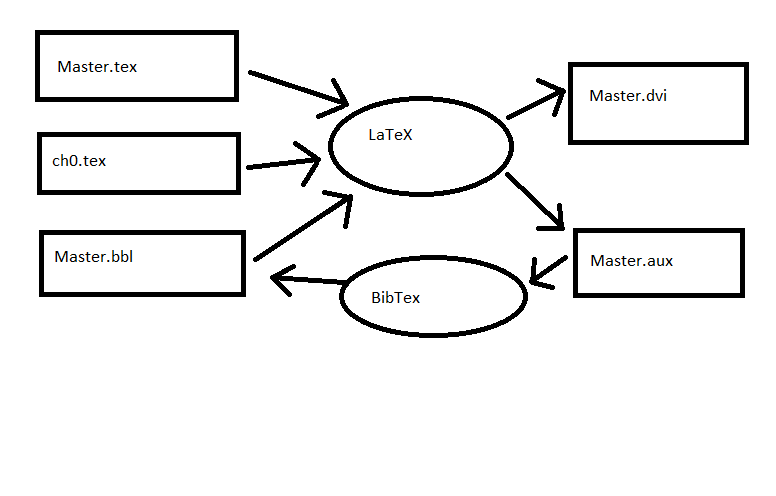
\includegraphics[
natheight=3.3062in, natwidth=5.1733in, height=3.352in, width=5.2295in]
{C:/Users/theo/Documents/munthesis/munthesis/graphics/figure__1.pdf}\caption{%
A simplified view of LaTeX bibligraphy generation.}\label{fig-bibtex}%
\end{figure}%
\fi
%EndExpansion
For example see Figure \ref{fig-bibtex}. I suggest sticking to PNG or EPS
for image formats.

To make the figure float, pick \textquotedblleft floating\textquotedblright\
from the \textquotedblleft layout\textquotedblright\ tab of its properties.
Select \textquotedblleft top of page\textquotedblright\ and
\textquotedblleft bottom\ of page\textquotedblright .

\subsection{Other Figures}

Any LaTeX can be a figure. The trick is to use \textquotedblleft TeX
Fields\textquotedblright\ and use LaTeX's figure environment the way I did
to produce Figure \ref{fig-eqn-as-figure}

%TCIMACRO{\TeXButton{B Figure}{\begin{figure}[tb]}}%
%BeginExpansion
\begin{figure}[tb]%
%EndExpansion
\begin{equation*}
\begin{array}{lll}
AP & \sqsubseteq & AS \\ 
\downarrow I &  & \downarrow I \\ 
CP & \sqsubseteq & CS%
\end{array}%
\end{equation*}

%TCIMACRO{%
%\TeXButton{E Figure}{\caption{A commutativity diagram}\label{fig-eqn-as-figure}
%\end{figure}}}%
%BeginExpansion
\caption{A commutativity diagram}\label{fig-eqn-as-figure}
\end{figure}%
%EndExpansion

To create a figure that is not based on an image file, use the fragment
\textquotedblleft figure\textquotedblright\ or, for single spacing,
\textquotedblleft ssfigure\textquotedblright .\footnote{%
A fragment is a snippet of text that has been saved to a file. To insert a
fragment use the fragment \textquotedblleft drop down\textquotedblright\
list or type Alt-4. Then pick the fragment you need.
\par
You can create your own fragments, by selecting some text and then File 
\TEXTsymbol{>}\TEXTsymbol{>}\ Save Fragment ...}

By the way there are several packages that make really fancy commutativity
diagrams. Figure \ref{fig-eqn-as-figure} simply uses a matrix (Insert 
\TEXTsymbol{>}\TEXTsymbol{>}\ Matrix --- which produces LaTeX's
\textquotedblleft array\textquotedblright\ environment) as a quick and dirty
way to make simple commutativity diagrams.

For really snazy figures you can use the TikZ package. See 
\begin{equation*}
\text{\url{http://www.texample.net/tikz/examples/all/}}
\end{equation*}

\noindent for lots of examples.

\subsection{Tables}

Scientific Word has good support for tables, but not for the floating kind.
To make floating tables, you can use \textquotedblleft TeX
Fields\textquotedblright\ and LaTeX's \textquotedblleft
table\textquotedblright\ environment.

To make his easier, I've created a fragment \textquotedblleft
sstable\textquotedblright\ that inserts a single spaced table.

See Table \ref{tab:cusses} for an example.

%TCIMACRO{\TeXButton{B Table}{\begin{table}[tb]}}%
%BeginExpansion
\begin{table}[tb]%
%EndExpansion
%TCIMACRO{\TeXButton{B SingleSpaced}{\begin{singlespaced}}}%
%BeginExpansion
\begin{singlespaced}%
%EndExpansion

\begin{equation*}
\begin{tabular}{|l|r|}
\hline
\textbf{Language} & \textbf{Cusses} \\ \hline\hline
C\# & 20 \\ \hline
C++ & 56 \\ \hline
C & 28 \\ \hline
Java & 20 \\ \hline
JavaScript & 46 \\ \hline
Perl & 30 \\ \hline
PHP & 4 \\ \hline
Python & 10 \\ \hline
Ruby & 53 \\ \hline
\end{tabular}%
\end{equation*}%
%TCIMACRO{\TeXButton{E SingleSpaced}{\end{singlespaced}}}%
%BeginExpansion
\end{singlespaced}%
%EndExpansion
%TCIMACRO{%
%\TeXButton{Caption}{\caption{Cuss count by programming language.}}}%
%BeginExpansion
\caption{Cuss count by programming language.}%
%EndExpansion
\label{tab:cusses}%
%TCIMACRO{\TeXButton{E Table}{\end{table}}}%
%BeginExpansion
\end{table}%
%EndExpansion

\section{Bibliography and Citations}

Use BibTeX to create your bibliography (or references) section. \ It is well
worth reading Oren Patashnik's manual for BibTeX \cite{Patashnik-1988}.
While BibTeX files can be edited with any text editor, I prefer to use
JabRef. However using JabRef or a similar tool is no replacement for reading
the manual. BibTeX has a number of peculiarities that it pays to be aware
of. Be particularly careful of BibTeX entries you obtain from sources such
as the ACM; these often exhibit a low standard of care.

Citations are inserted using Insert \TEXTsymbol{>}\TEXTsymbol{>}\ Typeset
Object \TEXTsymbol{>}\TEXTsymbol{>}\ Citation.

My favourite citation style is `Harvard style' or (\textquotedblleft
named\textquotedblright\ style) with square brackets. It looks like this

\begin{quotation}
LaTeX was created by Lamport \cite{Lamport-1994}.
\end{quotation}

If you don't like the way the author's name is sometimes repeated, as it is
in the preceding example, you can use the \texttt{\TEXTsymbol{\backslash}%
shortcite}, which shows only the year in brackets. You can enter such a
command as a \textquotedblleft TeX Field\textquotedblright\ (Menu Insert 
\TEXTsymbol{>}\TEXTsymbol{>}\ Typeset\ Object \TEXTsymbol{>}\TEXTsymbol{>}\
TeX Field). Or use the \textquotedblleft shortcite\textquotedblright\
fragment.

\begin{quotation}
LaTeX was created by Lamport 
%TCIMACRO{\TeXButton{Short Cite}{\shortcite{Lamport-1994}}}%
%BeginExpansion
\shortcite{Lamport-1994}%
%EndExpansion
.
\end{quotation}

\noindent This removes the temptation to do this sort of thing

\begin{quotation}
LaTeX was created by \cite{Lamport-1994}.
\end{quotation}

\noindent Which you should not do. (It suggests that LaTeX was created by a
book, which it was not.)\ Your sentences should read correctly with all
citations removed.

Many electrical and computer engineers use IEEE style, which is shorter, but
harder on the reader. It looks like this

\begin{quotation}
LaTeX was created by Lamport [1].
\end{quotation}

\noindent Some supervisors may insist on IEEE style. To get IEEE style
citations (and bibliography), double click on the BIBTEX field in the master
file and select an IEEE style. Then remove named.cite from the
\textquotedblleft Package Options\textquotedblright\ list for the master
document (Typeset \TEXTsymbol{>}\TEXTsymbol{>}\ Options and Packages 
\TEXTsymbol{>}\TEXTsymbol{>}\ Package Options).
}}%
%BeginExpansion
%TCIDATA{Version=5.50.0.2960}
%TCIDATA{LaTeXparent=0,0,Master.tex}
                      
%TCIDATA{ChildDefaults=chapter:1,page:1}


\chapter{Introduction}

\label{chap:intro}

\begin{comment}
The two TeX boxes on the following line should only be used for the first
chapter
\end{comment}

%TCIMACRO{\TeXButton{pagenumbering}{\pagenumbering{arabic}}}%
%BeginExpansion
\pagenumbering{arabic}%
%EndExpansion
%TCIMACRO{\TeXButton{Start at page 0}{\addtocounter{page}{-1}}}%
%BeginExpansion
\addtocounter{page}{-1}%
%EndExpansion

\begin{quotation}
\LaTeX is a system for typesetting documents. Its first widely available
version, mysteriously numbered 2.09, appeared in 1985. \LaTeX{} is now
extremely popular in the scientific and academic communities, and it is used
extensively in industry. It has become a \emph{lingua franca} of the
scientific world; scientists send their papers electronically to colleagues
around the world in the form of \LaTeX{} input.\cite{Lamport-1994}
\end{quotation}

\section{Getting started}

This document serves three purposes.

\begin{itemize}
\item It contains some information on how to use \LaTeX~\cite{Lamport-1994}
and Scientific Word to typeset your thesis.

\item It serves as a template that you can use for your thesis. Make a copy.

\item It contains many examples and some advice.
\end{itemize}

By default, all text is double spaced, however, lengthy quotations and
footnotes must be singled spaced. The left margin is slightly wider than the
right margin. This is to compensate for binding.

See \url{http://www.mun.ca/sgs/go/guid_policies/guidelines_intro.php} for
the SGS\ guidelines.

\section{Some tips, pitfalls, and opinions}

\label{sec:hints}

\subsection{Text mode}

\begin{itemize}
\item Use the View menu to turn on all the following:\ Invisibles, Helper
lines, Helper Boxes, Markers, Status Bar. Use View\ \TEXTsymbol{>}%
\TEXTsymbol{>}\ Toolbars to ensure that most tool bars are displayed. (I\
use all except History and Exam). Rearrange the tool bars with the mouse
until you are happy.

\item In text mode, type ` twice to get a \textquotedblleft\ and type '
twice to get \textquotedblright .

\item In LaTeX a closing single quotation mark and an apostrophe are the
same character. Use the ' key.

\item When you need three `s or three 's in a row, you can use a
\textquotedblleft zero space\textquotedblright\ (see below) to clarify what
is what. For example:\ John said, \textquotedblleft I heard her yell
`Stop'{}\textquotedblright . There is a zero space between the ' and the
\textquotedblright .

\item In text mode, type - twice to get and en-dash --. Type - three times
to get an em-dash --- . (Use en-dashes only for ranges of numbers or years.
Use em-dashes for punctuation.)

\item In text mode, the - key gives a hyphen, not a minus sign. Compare $x-y$
to \textit{x-y}.

\item For various kinds of horizontal spaces Insert \TEXTsymbol{>}%
\TEXTsymbol{>}\ Spacing \TEXTsymbol{>}\TEXTsymbol{>}\ Horizontal space (or
Alt i s h). See table \ref{tab-spaces} for more shortcuts and descriptions.

%TCIMACRO{\TeXButton{B}{\begin{table}[tbp] \centering}}%
%BeginExpansion
\begin{table}[tbp] \centering%
%EndExpansion
%TCIMACRO{\TeXButton{B SingleSpaced}{\begin{singlespaced}}}%
%BeginExpansion
\begin{singlespaced}%
%EndExpansion
$%
\begin{tabular}{|l|l|l|p{5cm}|}
\hline\hline
\multicolumn{1}{||l|}{\textbf{Space}} &  & \textbf{Shortcut} & 
\multicolumn{1}{|p{5cm}||}{\textbf{Use}} \\ \hline\hline
Normal & a b & Space bar & Text mode \\ \hline
Required & etc.\ a & Shift-space\  & Text mode, after a ., !, or ? that does
not end a sentence \\ \hline
Nonbreaking & Table~\ref{tab-spaces} & Cntl-space & Text mode, where a line
break would be confusing. \\ \hline
Em-space & a\quad b &  & Math or text mode. \\ \hline
2 em-space & a\qquad b &  & Math or text mode. \\ \hline
Thin space & $x\,y$ & Cntl-, & In math mode only. \\ \hline
Thick space & $x\;y$ & Cntl-Shift-space & In math mode only. \\ \hline
Italic correction & \textit{f}\/; &  & If needed, between italic and roman
characters. \\ \hline
Zero space & '{}\textquotedblright &  & Between ' and \textquotedblright\ or
` and \textquotedblleft . \\ \hline
Negative thin & $\cap \!\!\!\bullet $ &  & Math only. (Best to avoid the
need.) \\ \hline
No indent &  &  & Before a paragraph that should not be indented. \\ \hline
Custom &  &  & When long or stretchy spaces are needed. \\ \hline
\end{tabular}%
$%
%TCIMACRO{\TeXButton{E SingleSpaced}{\end{singlespaced}}}%
%BeginExpansion
\end{singlespaced}%
%EndExpansion
\caption{Horizontal spaces}\label{tab-spaces}%
%TCIMACRO{\TeXButton{E}{\end{table}}}%
%BeginExpansion
\end{table}%
%EndExpansion

\item You can double click on a space to change its width and nature. I\
find it easier to select the space and hit Control-F5

\item Tip:\ You can change the properties of spaces, letters, tables, and
other objects by selecting the object and hitting Control-F5.

\item Pitfall:\ Speaking of spaces. LaTeX will insert a little an
extra-stretchy space between sentences. About 99\% of the time\ LaTeX has no
problem correctly identifying the end of a sentence. The rule is this:\ Any
period (.), exclamation point (!), or question mark (?) that does not follow
a capital letter and that is followed by a normal space marks the end of a
sentence. So:

\begin{itemize}
\item When a period (.), exclamation point (!), or question mark (?) does
not end a sentence, follow it with a \textquotedblleft nonbreaking
space\textquotedblright\ (Alt i s h b) or a \textquotedblleft required
space\textquotedblright\ (Alt i s h r). For example, if I\ wrote
\textquotedblleft Dr.~N. loves C%
%TCIMACRO{\TeXButton{@}{\@}}%
%BeginExpansion
\@%
%EndExpansion
.\textquotedblright , I'd put a nonbreaking space between \textquotedblleft
Dr.\textquotedblright\ and \textquotedblleft N\textquotedblright . I could
have put a required space between the \textquotedblleft
N.\textquotedblright\ and \textquotedblleft loves\textquotedblright , but
there is no need, as LaTeX will assume that this period does not end a
sentence. I\ chose a nonbreaking space between \textquotedblleft
Dr.\textquotedblright\ and \textquotedblleft N.\textquotedblright\ because I
didn't want a line-break between them. For long surnames, it may be
preferable to use a required space after an abbreviated title.

\item When a period (.), exclamation point (!), or question mark (?) does
end a sentence but also follows a capital letter, put a LaTeX \TEXTsymbol{%
\backslash}@ command between the letter and the punctuation mark. For
example in \textquotedblleft Dr.~N. loves C%
%TCIMACRO{\TeXButton{@}{\@}}%
%BeginExpansion
\@%
%EndExpansion
.\textquotedblright , I'd put a LaTeX \TEXTsymbol{\backslash}@ command
between the \textquotedblleft C\textquotedblright\ and the \textquotedblleft
.\textquotedblright . Alt i y t can be used to insert a TeX command.\ Then
put \TEXTsymbol{\backslash}@ in the text box and click OK.

\item A common error is to put a normal space rather than a required space
after \textquotedblleft i.e.\textquotedblright , \textquotedblleft
e.g.\textquotedblright , \textquotedblleft etc.\textquotedblright\ If they
don't end a sentence, follow it by a required, rather than a normal space.
For example:\ \textquotedblleft CDC, Univac, etc.\ are no more, i.e.\
defunct.\textquotedblright

\item When a period (.), exclamation point (!), or question mark (?) is
followed by a close parenthesis, LaTeX will treat the parenthesis as the end
of the sentence and the following space will be extra stretchy.

\item When a period (.), exclamation point (!), or question mark (?) is
followed by a single or double close quotation mark, LaTeX should treat the
quotation mark as the end of a sentence. However, thanks to an SW oddity,
this won't work with SW. At present I have no good workaround.

\item The following table illustrates how LaTeX deals with various cases:%
%TCIMACRO{\TeXButton{B SingleSpaced}{\begin{singlespaced}}}%
%BeginExpansion
\begin{singlespaced}%
%EndExpansion
\begin{equation*}
\begin{tabular}{|l|p{3.2cm}|}
\hline
Default behaviour & \textquotedblleft (M M m. M MMMM. \\ \hline
Required space & \textquotedblleft (M M m.\ M MMMM. \\ \hline
Paren after period & \textquotedblleft M M m.) M MMMM. \\ \hline
Quote after period. & (M M m.\textquotedblright\ M MMMM. \\ \hline
Period after capital. & \textquotedblleft (m M M. M MMMM. \\ \hline
\TEXTsymbol{\backslash}@ before period & \textquotedblleft (m M M%
%TCIMACRO{\TeXButton{@}{\@}}%
%BeginExpansion
\@%
%EndExpansion
. M MMMM. \\ \hline
\end{tabular}%
\end{equation*}%
%TCIMACRO{\TeXButton{E SingleSpaced}{\end{singlespaced}}}%
%BeginExpansion
\end{singlespaced}%
%EndExpansion
\end{itemize}

\item The `Noindent space' (Insert \TEXTsymbol{>}\TEXTsymbol{>}\ Spacing 
\TEXTsymbol{>}\TEXTsymbol{>}\ Horizontal Space... \TEXTsymbol{>}\TEXTsymbol{>%
}\ Noindent or Alt i s h n) is not really a space at all. It can be used at
the start of a paragraph to suppress its indentation. This is useful when a
list is used that is not at the end of a paragraph.

\item Usually TeX hyphenates without trouble. If it fails to hyphenate \emph{%
Entscheidungsproblem}, for example, correctly you can indicate all the
places where it can hyphenate such troublesome words, using Insert 
\TEXTsymbol{>}\TEXTsymbol{>}\ Spacing \TEXTsymbol{>}\TEXTsymbol{>}\ Break 
\TEXTsymbol{>}\TEXTsymbol{>}\ Discretionany Hyphen.

\item To indicate where line breaks are allowed insert an \textquotedblleft
allow break\textquotedblright\ command (Insert \TEXTsymbol{>}\TEXTsymbol{>}\
Spacing \TEXTsymbol{>}\TEXTsymbol{>}\ Break \TEXTsymbol{>}\TEXTsymbol{>}\
Allow break or Alt i s b a). For example, if I give a file name as
/usr/\allowbreak theo/\allowbreak docs/\allowbreak thesis/\allowbreak
Master.tex. I\ might do well to add an `allow break' after each / except the
first.

\item For URLs and URIs use, Insert \TEXTsymbol{>}\TEXTsymbol{>} TeX Object 
\TEXTsymbol{>}\TEXTsymbol{>} Tex Field ... and insert \texttt{\TEXTsymbol{%
\backslash}url\{\emph{your url}\}}. Follow the link %
\url{http://en.wikibooks.org/wiki/LaTeX/Hyperlinks} for more. This has
several advantages:\ It correctly typesets characters such as tildes. It
allows breaks at the right places. It sets the URL in typewriter font. It
will insert actual hyperlinks into the PDF copy of your thesis, if you
compile it with PDFLaTeX.
\end{itemize}

\subsection{Math mode}

\begin{itemize}
\item Control-m will switch to math mode. Control-t will switch to text mode.

\item I\ set up my User Setup (Tools \TEXTsymbol{>}\TEXTsymbol{>} User
setup) so that the spacebar after a space will switch from text mode to math
mode and a spacebar while in math mode will switch to text mode. That way,
two taps on the spacebar will switch modes and insert a space.

\item To get spaces in math mode, use Control-Shift-Spacebar to get a thick
space $f\;x$ and Control-Comma to get a thin space $f\,x$.

\item In math mode, the - key gives a minus sign, not a hyphen. Compare $x-y$
to \textit{x-y}.

\item In math-mode ' gives you a superscript prime. Compare \textit{x'} to $%
x^{\prime }$. If you really need an apostrophe, closing single quote, or
double quote, switch to text mode.

\item Control-d will insert a new math display as shown in (\ref{eqn:example}%
) 
\begin{equation}
\left( 
\begin{array}{c}
k \\ 
3%
\end{array}%
\right) +\frac{\left( 
\begin{array}{c}
k \\ 
2%
\end{array}%
\right) \left( 
\begin{array}{c}
k-2 \\ 
2%
\end{array}%
\right) }{2}=\frac{1}{(k-2)!}\ \sum_{i=0}^{k-3}(-1)^{i}\left( 
\begin{array}{c}
k-2 \\ 
i%
\end{array}%
\right) (k-2-i)^{k}\text{\quad .}  \label{eqn:example}
\end{equation}

\item When your insertion point (i.e.~caret) is in a math display, the tab
key will toggle whether the display is numbered. Double clicking to the left
or right the display will then bring up a \textquotedblleft display
properties dialog\textquotedblright\ where the \textquotedblleft
key\textquotedblright\ (i.e., \textquotedblleft label\textquotedblright )
can be set. The key is then used in cross references.

\item Multiple line math displays can have separate numbers for each line
and each number is optional. For example%
\begin{eqnarray}
&&\left. f\sqsubseteq g;h\right.   \label{eq:wpreLHS} \\
&=&  \notag \\
&&\left. h\backslash f\sqsubseteq g\right.   \label{eq:wpreRHS}
\end{eqnarray}

\item Opinion:\ Displays should be used when a formula might cause a bad
line break, when the formula is so tall that it will cause an irregular
distance between lines of text, when a formula is long, or when it needs a
number.

\item Opinion: It is good style to only number those displays that need to
be referred to in the text. I.e., that will be cross referenced.

\item Opinion:\ Usually it is best to \textbf{not} omit punctuation after
displayed math. I\ usually leave an em-space or a quad-space between the
math and the punctuation. For example:\ Now it is time to prove%
\begin{equation*}
P\sqsubseteq Q\text{\quad .}
\end{equation*}%
I make an exception\ for computer code. For example:\ 
\begin{equation*}
\text{\texttt{rm -r -f tmp}\quad .}
\end{equation*}%
If the period at the end of that sentence were ,misunderstood to be part of
the code, the meaning of the code would change considerably. The IEEE style
guide suggests omitting the period at the end of sentence, but not other
punctuation.

\item Pitfall: After a display, be careful to only start a new paragraph if
you need one.

\item Pitfall: Multi-character identifiers should not be set in math mode's
default italic font, like this $\sin (first)$. Instead use the \textit{italic%
} font, like this $\sin (\mathit{first})$. The reason is that TeX uses
slightly different fonts for \textquotedblleft math
italic\textquotedblright\ and \textquotedblleft italic\textquotedblright .
The math italic font is designed so that the spacing between adjacent
letters is correct for implicit multiplication or function application $xy+fx
$. The italic font is designed so the letter spacing is correct for words.
(I\ have set Shift-F6 to give \textit{italic font}.)

\item Opinion:\ I\ generally use italic (or math italic, if only one letter
is used)\ for variables and \textrm{an upright font such as Roman}
(Shift-F4) or \textsf{sans-serif} (Shift-F5) for constants, e.g. $\sin (x)$,
but $f(\mathrm{e})$. However, as Alan Perlis once said, \textquotedblleft
one man's constant is another man's variable\textquotedblright . If a
certain sequence of letters is intended to represent exactly the same thing
everywhere in your thesis, it's probably a constant. Otherwise, it is
probably a variable. (Aside:\ Strictly speaking, the opinion that constants
should be set upright should be applied to $e$, $i$, and $\pi $.\ However,
it is not easy to make an upright $\pi $ with Scientific Word, as the
required fonts are not included. The best I can do is $\mathrm{e}^{\mathrm{i}%
\pi }+1=0$.)

\item Use Control-( to enter a pair of round brackets\ (parenthesis) $\left(
x\right) $, Control-[ for square brackets $\left[ x\right] $, Control-\{ for
curly brackets (braces) $\left\{ x\right\} $, Control-\TEXTsymbol{<} for
angle brackets $\left\langle x\right\rangle $, Control-\TEXTsymbol{\backslash%
} for absolute values $\left\vert x\right\vert $, and Control-\TEXTsymbol{%
\vert} for norms $\left\Vert x\right\Vert $. Use Insert \TEXTsymbol{>}%
\TEXTsymbol{>}\ Brackets (for any other combinations such as $\left\lceil
x\right\rfloor $.

\item Opinion:\ Bracket pairs entered this way will automatically enlarge.
Compare 
\begin{equation*}
\left( \frac{fx}{gx},hx\right) \text{ to }(\frac{fx}{gx},hx)
\end{equation*}%
The former is preferable.

\item However, avoid such \textquotedblleft paired
brackets\textquotedblright\ in in-line math (as opposed to displayed math).
The reason is that, LaTeX will not insert a line break between paired
brackets. If the brackets need to be enlarged, the formula, should likely
have been in a display anyway.

\item Opinion:\ Never use $\left[ {}\right] $ or $\left\{ {}\right\} $
brackets for simple grouping. E.g., $u\times \left( v+\left( w+\left(
xy\right) \right) \right) $ is preferable to $u\times \left\{ v+\left[
w+\left( xy\right) \right] \right\} $; the curly $\left\{ {}\right\} $
bracket should be used for sets and the square $\left[ {}\right] $ brackets
often have some meaning ascribed to them, for example, sequencing.

\item Never use less-than and greater-than signs in place of angle brackets.
Not only are they the wrong symbols, but LaTeX puts too much space or too
little space around them. Compare $P=<x^{\prime }=x>$ to $P=\left\langle
x^{\prime }=x\right\rangle $.

\item Invisible brackets (use Insert \TEXTsymbol{>}\TEXTsymbol{>}\ Brackets)
are useful sometimes. For example if I\ want to define a relation I\ might
use%
\begin{align*}
\left. f\equiv g\right. & \triangleq f\sqsubseteq g\wedge f\sqsubseteq g \\
f^{\smallsmile }& \triangleq \lambda s\lambda s^{\prime }\cdot f\,s^{\prime
}\,s
\end{align*}%
There are invisible brackets around $f\equiv g$ so that the vertical
alignment and the horizontal spacing is correct. Also use an invisible
bracket for cases:%
\begin{equation*}
f(x)=\left\{ 
\begin{array}{lll}
g(x) & \qquad  & \text{if }x>0 \\ 
h(x) &  & \text{otherwise}%
\end{array}%
\right. 
\end{equation*}

\item Use Control-$\downarrow $ and Control-$\uparrow $ for sub- and
superscripts $x_{i_{j}}^{2}$. Use the spacebar or $\rightarrow $ key to exit
the sub- or superscript.

\item Opinion: It is generally bad style to over use subscripts. If you ever
find you need two levels of sub(or super)scripts, rethink your notation.

\item Use markers (labels)\ and cross-references to refer numbered displays
(see (\ref{eqn:example}) on page \pageref{eqn:example}), sections (see
section \ref{sec:sections} on page \pageref{sec:sections}), figures and
tables. To enter a new marker\ (label) use the \textquotedblleft
Marker\textquotedblright\ button on the \textquotedblleft
Field\textquotedblright\ toolbar or Insert \TEXTsymbol{>}\TEXTsymbol{>}
Marker ... (Alt i e). To enter a cross-reference use \textquotedblleft Cross
Reference\textquotedblright\ button on the \textquotedblleft Typeset
object\textquotedblright\ toolbar or Insert\ \TEXTsymbol{>}\TEXTsymbol{>}\
Typeset Object \TEXTsymbol{>}\TEXTsymbol{>} Cross Reference ... (Alt i y r).
When you insert or edit a cross reference, markers in other chapters won't
show up in the list of markers; that's ok; just type in the marker.

\item Tip:\ Abbreviate frequently used symbols in math mode with automatic
substitutions (Tools \TEXTsymbol{>}\TEXTsymbol{>} Automatic Substitutions).
Develop your own system of substitutions that is easy for you to remember.
Unfortunately only letters can be used, so you can't start your
abbreviations with, say, a \TEXTsymbol{\backslash} . I\ use the letter q to
start many of my abbreviations. E.g. qa for $\wedge $, qo for $\vee $, qrb
for $\sqsubseteq $, and so on.

\item Table \ref{tab:keys} summarizes some of useful key combinations for
editing math. 
%TCIMACRO{\TeXButton{B}{\begin{table}[tbp] \centering}}%
%BeginExpansion
\begin{table}[tbp] \centering%
%EndExpansion
%TCIMACRO{\TeXButton{B SingleSpaced}{\begin{singlespaced}}}%
%BeginExpansion
\begin{singlespaced}%
%EndExpansion
\begin{tabular}{|l|l|}
\hline\hline
\multicolumn{1}{||l|}{\textbf{Key}} & \multicolumn{1}{|l||}{\textbf{Meaning}}
\\ \hline\hline
Control-m & Math mode \\ \hline
Control-t & Text mode \\ \hline
Control-d & Displayed math \\ \hline
Tab & Toggle display numbering \\ \hline
Tab & Go to next input box \\ \hline
Control-Shift-spacebar & Thick math space \\ \hline
Control-, & Thin math space \\ \hline
Control-g letter & Greek letter \\ \hline
Control-s letter & Symbol. E.g. Control-s v gives $\vee $ \\ \hline
Control-/ & Fraction $\frac{x}{y}$ \\ \hline
Control-(, Control-9 & $\left( x\right) $ \\ \hline
Control-[ & $\left[ x\right] $ \\ \hline
Control-\{ & $\left\{ x\right\} $ \\ \hline
Control-\TEXTsymbol{\backslash} & $\left\vert x\right\vert $ \\ \hline
Control-\TEXTsymbol{\vert} & $\left\Vert x\right\Vert $ \\ \hline
Control-\TEXTsymbol{<} & $\left\langle x\right\rangle $ \\ \hline
Control-$\downarrow $ & $x_{y}$ \\ \hline
Control-$\uparrow $ & $x^{y}$ \\ \hline
\end{tabular}%
%TCIMACRO{\TeXButton{E SingleSpaced}{\end{singlespaced}}}%
%BeginExpansion
\end{singlespaced}%
%EndExpansion
\caption{Some useful keys}\label{tab:keys}%
%TCIMACRO{\TeXButton{E}{\end{table}}}%
%BeginExpansion
\end{table}%
%EndExpansion
\end{itemize}

\subsection{Function keys}

Table \ref{tab:fkeys} on page \pageref{tab:fkeys} summarizes some useful
functions keys. You can reprogram most function keys with Tag \TEXTsymbol{>}%
\TEXTsymbol{>}\ Function Keys... Table \ref{tab:keys} on page \pageref%
{tab:keys} gives some other useful key combinations

%TCIMACRO{\TeXButton{B}{\begin{table}[tbp] \centering}}%
%BeginExpansion
\begin{table}[tbp] \centering%
%EndExpansion
%TCIMACRO{\TeXButton{B SingleSpaced}{\begin{singlespaced}}}%
%BeginExpansion
\begin{singlespaced}%
%EndExpansion
\begin{tabular}{|l|l|}
\hline\hline
\multicolumn{1}{||l|}{\textbf{Function Key}} & \multicolumn{1}{|l||}{\textbf{%
Meaning}} \\ \hline\hline
F1 & Help \\ \hline
F2 & Pop the top item tag \\ \hline
F3 & Body Text \\ \hline
F4 & Clear font \\ \hline
Shift-F4 & \textrm{Roman font} \\ \hline
F5 & \textbf{Bold} \\ \hline
Shift-F5 & \textsf{Sans-serif font} \\ \hline
Control-F5 & Edit Properties \\ \hline
F6 & \emph{Emphasis} \\ \hline
Shift-F6 & \textit{Italic font} \\ \hline
F7 & Numbered item \\ \hline
Shift-F7 & Indent code \\ \hline
F8 & Bullet item \\ \hline
Shift-F8 & Code \\ \hline
F9 & \texttt{Typewriter font} \\ \hline
Shift-F9 & $\mathcal{CALIGRAPHIC~FONT}$ \\ \hline
F10 & Access menu \\ \hline
F11 & Section \\ \hline
F12 & Subsection \\ \hline
Shift-F11 & Subsubsection \\ \hline
Shift-F12 & Sub$^{3}$section \\ \hline
\end{tabular}%
%TCIMACRO{\TeXButton{E SingleSpaced}{\end{singlespaced}}}%
%BeginExpansion
\end{singlespaced}%
%EndExpansion
\caption{Some useful function keys}\label{tab:fkeys}%
%TCIMACRO{\TeXButton{E}{\end{table}}}%
%BeginExpansion
\end{table}%
%EndExpansion

\section{Figures and Tables}

\subsection{Figures from image files}

Scientific Workplace has good support for figures if they come from an image
file. Use File \TEXTsymbol{>}\TEXTsymbol{>}\ Import Picture... or Alt-f-i 
%TCIMACRO{%
%\FRAME{ftbFU}{5.2295in}{3.352in}{0pt}{\Qcb{A simplified view of LaTeX bibligraphy generation.}}{\Qlb{fig-bibtex}}{figure.png}{%
%\special{language "Scientific Word";type "GRAPHIC";maintain-aspect-ratio TRUE;display "USEDEF";valid_file "F";width 5.2295in;height 3.352in;depth 0pt;original-width 5.1733in;original-height 3.3062in;cropleft "0";croptop "1";cropright "1";cropbottom "0";filename 'graphics/figure.png';file-properties "XNPEU";}}}%
%BeginExpansion
\ifcase\msipdfoutput
\FRAME{ftbFU}{5.2295in}{3.352in}{0pt}{\Qcb{A simplified view of LaTeX
bibligraphy generation.}}{\Qlb{fig-bibtex}}{figure.png}{%
\special{language "Scientific Word";type "GRAPHIC";maintain-aspect-ratio
TRUE;display "USEDEF";valid_file "F";width 5.2295in;height 3.352in;depth
0pt;original-width 5.1733in;original-height 3.3062in;cropleft "0";croptop
"1";cropright "1";cropbottom "0";filename
'graphics/figure.png';file-properties "XNPEU";}}%
\else
\begin{figure}[tb]\centering
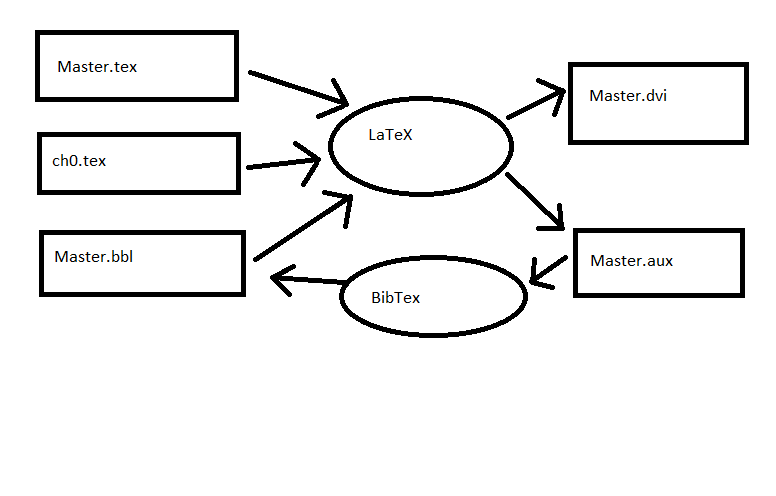
\includegraphics[
natheight=3.3062in, natwidth=5.1733in, height=3.352in, width=5.2295in]
{C:/Users/theo/Documents/munthesis/munthesis/graphics/figure__1.pdf}\caption{%
A simplified view of LaTeX bibligraphy generation.}\label{fig-bibtex}%
\end{figure}%
\fi
%EndExpansion
For example see Figure \ref{fig-bibtex}. I suggest sticking to PNG or EPS
for image formats.

To make the figure float, pick \textquotedblleft floating\textquotedblright\
from the \textquotedblleft layout\textquotedblright\ tab of its properties.
Select \textquotedblleft top of page\textquotedblright\ and
\textquotedblleft bottom\ of page\textquotedblright .

\subsection{Other Figures}

Any LaTeX can be a figure. The trick is to use \textquotedblleft TeX
Fields\textquotedblright\ and use LaTeX's figure environment the way I did
to produce Figure \ref{fig-eqn-as-figure}

%TCIMACRO{\TeXButton{B Figure}{\begin{figure}[tb]}}%
%BeginExpansion
\begin{figure}[tb]%
%EndExpansion
\begin{equation*}
\begin{array}{lll}
AP & \sqsubseteq & AS \\ 
\downarrow I &  & \downarrow I \\ 
CP & \sqsubseteq & CS%
\end{array}%
\end{equation*}

%TCIMACRO{%
%\TeXButton{E Figure}{\caption{A commutativity diagram}\label{fig-eqn-as-figure}
%\end{figure}}}%
%BeginExpansion
\caption{A commutativity diagram}\label{fig-eqn-as-figure}
\end{figure}%
%EndExpansion

To create a figure that is not based on an image file, use the fragment
\textquotedblleft figure\textquotedblright\ or, for single spacing,
\textquotedblleft ssfigure\textquotedblright .\footnote{%
A fragment is a snippet of text that has been saved to a file. To insert a
fragment use the fragment \textquotedblleft drop down\textquotedblright\
list or type Alt-4. Then pick the fragment you need.
\par
You can create your own fragments, by selecting some text and then File 
\TEXTsymbol{>}\TEXTsymbol{>}\ Save Fragment ...}

By the way there are several packages that make really fancy commutativity
diagrams. Figure \ref{fig-eqn-as-figure} simply uses a matrix (Insert 
\TEXTsymbol{>}\TEXTsymbol{>}\ Matrix --- which produces LaTeX's
\textquotedblleft array\textquotedblright\ environment) as a quick and dirty
way to make simple commutativity diagrams.

For really snazy figures you can use the TikZ package. See 
\begin{equation*}
\text{\url{http://www.texample.net/tikz/examples/all/}}
\end{equation*}

\noindent for lots of examples.

\subsection{Tables}

Scientific Word has good support for tables, but not for the floating kind.
To make floating tables, you can use \textquotedblleft TeX
Fields\textquotedblright\ and LaTeX's \textquotedblleft
table\textquotedblright\ environment.

To make his easier, I've created a fragment \textquotedblleft
sstable\textquotedblright\ that inserts a single spaced table.

See Table \ref{tab:cusses} for an example.

%TCIMACRO{\TeXButton{B Table}{\begin{table}[tb]}}%
%BeginExpansion
\begin{table}[tb]%
%EndExpansion
%TCIMACRO{\TeXButton{B SingleSpaced}{\begin{singlespaced}}}%
%BeginExpansion
\begin{singlespaced}%
%EndExpansion

\begin{equation*}
\begin{tabular}{|l|r|}
\hline
\textbf{Language} & \textbf{Cusses} \\ \hline\hline
C\# & 20 \\ \hline
C++ & 56 \\ \hline
C & 28 \\ \hline
Java & 20 \\ \hline
JavaScript & 46 \\ \hline
Perl & 30 \\ \hline
PHP & 4 \\ \hline
Python & 10 \\ \hline
Ruby & 53 \\ \hline
\end{tabular}%
\end{equation*}%
%TCIMACRO{\TeXButton{E SingleSpaced}{\end{singlespaced}}}%
%BeginExpansion
\end{singlespaced}%
%EndExpansion
%TCIMACRO{%
%\TeXButton{Caption}{\caption{Cuss count by programming language.}}}%
%BeginExpansion
\caption{Cuss count by programming language.}%
%EndExpansion
\label{tab:cusses}%
%TCIMACRO{\TeXButton{E Table}{\end{table}}}%
%BeginExpansion
\end{table}%
%EndExpansion

\section{Bibliography and Citations}

Use BibTeX to create your bibliography (or references) section. \ It is well
worth reading Oren Patashnik's manual for BibTeX \cite{Patashnik-1988}.
While BibTeX files can be edited with any text editor, I prefer to use
JabRef. However using JabRef or a similar tool is no replacement for reading
the manual. BibTeX has a number of peculiarities that it pays to be aware
of. Be particularly careful of BibTeX entries you obtain from sources such
as the ACM; these often exhibit a low standard of care.

Citations are inserted using Insert \TEXTsymbol{>}\TEXTsymbol{>}\ Typeset
Object \TEXTsymbol{>}\TEXTsymbol{>}\ Citation.

My favourite citation style is `Harvard style' or (\textquotedblleft
named\textquotedblright\ style) with square brackets. It looks like this

\begin{quotation}
LaTeX was created by Lamport \cite{Lamport-1994}.
\end{quotation}

If you don't like the way the author's name is sometimes repeated, as it is
in the preceding example, you can use the \texttt{\TEXTsymbol{\backslash}%
shortcite}, which shows only the year in brackets. You can enter such a
command as a \textquotedblleft TeX Field\textquotedblright\ (Menu Insert 
\TEXTsymbol{>}\TEXTsymbol{>}\ Typeset\ Object \TEXTsymbol{>}\TEXTsymbol{>}\
TeX Field). Or use the \textquotedblleft shortcite\textquotedblright\
fragment.

\begin{quotation}
LaTeX was created by Lamport 
%TCIMACRO{\TeXButton{Short Cite}{\shortcite{Lamport-1994}}}%
%BeginExpansion
\shortcite{Lamport-1994}%
%EndExpansion
.
\end{quotation}

\noindent This removes the temptation to do this sort of thing

\begin{quotation}
LaTeX was created by \cite{Lamport-1994}.
\end{quotation}

\noindent Which you should not do. (It suggests that LaTeX was created by a
book, which it was not.)\ Your sentences should read correctly with all
citations removed.

Many electrical and computer engineers use IEEE style, which is shorter, but
harder on the reader. It looks like this

\begin{quotation}
LaTeX was created by Lamport [1].
\end{quotation}

\noindent Some supervisors may insist on IEEE style. To get IEEE style
citations (and bibliography), double click on the BIBTEX field in the master
file and select an IEEE style. Then remove named.cite from the
\textquotedblleft Package Options\textquotedblright\ list for the master
document (Typeset \TEXTsymbol{>}\TEXTsymbol{>}\ Options and Packages 
\TEXTsymbol{>}\TEXTsymbol{>}\ Package Options).
%
%EndExpansion

\begin{comment}
Add more chapters here:\ Use Insert \TEXTsymbol{>}\TEXTsymbol{>}\ Typeset
Object \TEXTsymbol{>}\TEXTsymbol{>} Subdocument ...
\end{comment}

%TCIMACRO{\QSubDoc{Include chTags}{%TCIDATA{Version=5.50.0.2960}
%TCIDATA{LaTeXparent=0,0,Master.tex}
                      
%TCIDATA{ChildDefaults=chapter:1,page:1}


\chapter{Tags and environments\label{chap:tags}}

In order to use tags, the Tag toolbar should be showing (View \TEXTsymbol{>}%
\TEXTsymbol{>}\ Toolbars). This toolbar has 3 \textquotedblleft
drop-down\textquotedblright\ menus.

\begin{itemize}
\item Item Tags (Alt-1)

\item Section/Body Tags (Alt-2)

\item Text\ Tags\ (Alt-3)
\end{itemize}

\section{Sections and Chapters\label{sec:sections}}

Chapters:\ No function key is assigned to chapter heads. Use the
Section/Body Tag drop-down (Alt-2).

F11 gives a new section head

\subsection{Subsections}

F12 gives a new subsection

\subsubsection{Subsubsections}

Shift-F11 gives a new subsubsection

\paragraph{Subsubsubsections}

Shift-F12 gives a new sub$^{3}$section (aka a paragraph). These are not
numbered and do not appear in the Table of\ Contents.

\section{Body tags}

The Section/Body tag drop-down (Alt-2) is used for environments that
typically do not nest and section headings. We've seen section headings
above. Some of the other environments available via Section/Body tags are

F3 Body text. This is the default kind of paragraph

\begin{center}
Centred. It was our yesterdayes resolution, and agreement, that we should to
day discourse the most distinctly, and particularly we could possible, of
the natural reasons, and their efficacy that have been hitherto alledged on
the one or other part, by the maintainers of the Positions, Aristotelian,
and Ptolomaique; and by the followers of the Copernican Systeme:
\end{center}

\begin{flushleft}
Flush left. And because Copernicus placing the Earth among the moveable
Bodies of Heaven, comes to constitute a Globe for the same like to a Planet;
it would be good that we began our disputation with the examination of what,
and how great the energy of the Peripateticks arguments is, when they
demonstrate, that this Hypothesis is impossible:
\end{flushleft}

\begin{flushright}
Flush right. Since that it is necessary to introduce in Nature, substances
different betwixt themselves, that is, the C\oe lestial, and Elementathat
impassible and immortal, this alterable and corruptible. Which argument
Aristotle handleth in his book De C\oe lo, insinuating it first, by some
discourses dependent on certain general assumptions, and afterwards
confirming it with experiments and perticular demonstrations: following the
same method, I will propound, and freely speak my judgement, submitting my
self to your censure, and particularly to Simplicius, a Stout Champion and
contender for the Aristotelian Doctrine.
\end{flushright}

\begin{quotation}
Long quotation. And the first Step of the Peripatetick arguments is that,
where Aristotle proveth the integrity and perfection of the World, telling
us, that it is not a simple line, nor a bare superficies, but a body adorned
with Longitude, Latitude, and Profundity.
\end{quotation}

\begin{quote}
Short Quote.
\end{quote}

Body and section tags should be applied only to top-level paragraphs.
Furthermore Item tags can not be used within Body tags. You can try to make
a list of quotations or a quotation that contains a list, but the
straight-forward approach is not likely to succeed. (These things can be
done with LaTeX; the limitation is with Scientific Word and Scientific
Workplace.)

\section{Item tags and environments that nest}

The \textquotedblleft Item Tag\textquotedblright\ drop-down (Alt-1) lists
all tags that nest. Some of these generate list-like environments in LaTeX.

\begin{itemize}
\item Bullet lists F8

\begin{enumerate}
\item Numbered lists F7

\begin{description}
\item[Description lists:] Use \textquotedblleft Description List
Item\textquotedblright\ on the Item Tag drop down.

\item[Depth:] You can nest item tags to a depth of 4, but no more

\begin{itemize}
\item This list item is at depth 4. LaTeX supports deeper nesting, but
Scientific Word and WorkPlace do not.
\end{itemize}
\end{description}

\item See also the \textquotedblleft code\textquotedblright\ and
\textquotedblleft indent\textquotedblright\ tags discussed in the next
chapter.
\end{enumerate}

\item F2 to step out a level.

\item 
%TCIMACRO{\TeXButton{B SingleSpaced}{\begin{singlespaced}}}%
%BeginExpansion
\begin{singlespaced}%
%EndExpansion
The \textquotedblleft singlespaced\textquotedblright\ environment is not
associated with a function key or tag. You can use TeX fields (Insert\ 
\TEXTsymbol{>}\TEXTsymbol{>}\ Typeset Object \TEXTsymbol{>}\TEXTsymbol{>}
TeX Field) to insert the required LaTeX magic. You can also use the
\textquotedblleft singlespaced\textquotedblright\ fragment.%
%TCIMACRO{\TeXButton{E SingleSpaced}{\end{singlespaced}}}%
%BeginExpansion
\end{singlespaced}%
%EndExpansion
\end{itemize}

\section{Theorems and proofs}

Theorem-like environments and proofs (perhaps surprisingly) nest. Use the
Item Tag drop-down (Alt-1) Be sure to use F2 (Remove Item Tag) after the end
of each.

\begin{axiom}[The axiom of equality]
All animals are equal.
\end{axiom}

\begin{claim}
That some animals are more equal than others.
\end{claim}

\begin{conclusion}
Whatever goes upon two legs is an enemy.
\end{conclusion}

\begin{condition}
No animal shall drink alcohol.
\end{condition}

\begin{corollary}
Whatever goes upon four legs, or has wings, is a friend.
\end{corollary}

\begin{conjecture}
All men are enemies. All animals are comrades.
\end{conjecture}

\begin{criterion}
No animal shall kill any other animal.
\end{criterion}

\begin{definition}[Insanity]
Doing the same thing over and over again while expecting different results.
\end{definition}

\begin{example}
Example is not the main thing in influencing others. It is the only thing.
\end{example}

\begin{exercise}
Find all errors in Cantor's diagonal proof that the continuum is larger than 
$\aleph _{0}$.
\end{exercise}

\begin{lemma}
What is yellow and equivalent to the axiom of choice. ... Zorn's Lemon.
\end{lemma}

\begin{notation}
We use $\left\langle E\right\rangle $ to represent that total function $f$
in $\Sigma \times \Sigma \rightarrow \mathbb{B}$ such that $f(\sigma ,\sigma
^{\prime })$ is equal to the value of the expression obtained by replacing,
in the boolean expression $E$, each unprimed identifier $i$ with $\sigma .i$
and each primed identifier $i^{\prime }$ with $\sigma ^{\prime }.i$.
\end{notation}

\begin{problem}
Show that $P=NP$ or that $P\neq NP$.
\end{problem}

\begin{proposition}
No animal shall wear clothes.
\end{proposition}

\begin{solution}
That which is not in the problem set is in the solution set.
\end{solution}

\begin{summary}
No question now, what had happened to the faces of the pigs. The creatures
outside looked from pig to man, and from man to pig, and from pig to man
again; but already it was impossible to say which was which.
\end{summary}

\begin{theorem}[The Curry/L\"{o}b paradox]
\label{thm:santa}I am Santa Claus.
\end{theorem}

\begin{remark}
Truth is an ill-defined concept.
\end{remark}

\begin{proof}
(Theorem \ref{thm:santa}.)

(a)\ Let $S$ be the statement \textquotedblleft If $S$ is true, then I am
Santa Claus\textquotedblright .

(b)\ Assume, for the moment that $S$ is true.

\begin{itemize}
\item Since $S$ is true and $S$ is the statement \textquotedblleft If $S$ is
true, then I am Santa Claus\textquotedblright , the statement
\textquotedblleft If $S$ is true, then I am Santa Claus\textquotedblright\
is true.

\item Therefore, if $S$ is true, then I am Santa Claus.

\item As we are assuming $S$ is true, I\ am (under that assumption)\ Santa
Claus.
\end{itemize}

(c) Since in (b), assuming $S$ to be true lead to the conclusion that I am
Santa Claus, we can see that \textquotedblleft If $S$ is true, then I am
Santa Claus\textquotedblright\ is true.

(d)\ By (c)\ and (a), $S$ is true.

(e)\ From (c), if $S$ is true, then I am Santa Claus.

(f)\ From (d) and (e), by modus ponens, I am Santa Claus.
\end{proof}

In Scientific Word and WorkPlace you can double click the tagged paragraph's
leader (i.e. the word(s) or symbols leading the paragraph) to enter an
optional \textquotedblleft custom label\textquotedblright ,\ as I\ did with
the Axiom, Definition, and Theorem above. This works for theorem-like
environments and description-list items. It does not work for proofs.

The numbering system that I have chosen is to number theorems sequentially
within each chapter and all other theorem-like entities as if they were also
theorems. You can use another numbering system if you want; to do so, edit
the preamble (Typeset \TEXTsymbol{>}\TEXTsymbol{>}\ Preamble) of the master
document.

\section{Fonts and sizes}

The Text Tag drop-down (Alt-3) is used for tags that operate at the
character level rather than the paragraph level.

\begin{itemize}
\item F4 to return to the default.

\item \textrm{Shift-F4 for roman}

\item \textbf{F5 for bold}

\item \textsf{Shift-F5 for sans-serif}

\item \emph{F6 for emphasized. Emphasized (by default) alternates between
italic and upright as it nests}

\item \textit{Shift-F6 for italic. Italic is always italic. Use italic for
multi-letter names in math mode.}

\item \texttt{F9 for typewriter}

\item $\mathcal{SHIFT}$-$\mathcal{F}9~\mathcal{FOR\ CALIGRAPHIC}$ Only
capitals and numerals. Best saved for math.

\item $\mathfrak{Frackur}$ Best saved for math

\item $\mathbb{BLACKBOARD\ BOLD}$ Only capitals. Use only for constant sets: 
$\mathbb{C}$ for the complex numbers, $\mathbb{R}$ for the real numbers, $%
\mathbb{Z}$ for the integers, $\mathbb{N}$ for the natural numbers, $\mathbb{%
B}$ for the Booleans.

\item \textsc{Small Capitals}.

\item Most font size changes needed are done automatically. You should never
or only very rarely use {\Huge size} {\scriptsize changing} {\LARGE text} 
{\tiny tags}.

\item \emph{\textbf{Combining text tags is possible, but rather tricky,
unless one tag is strictly within the other. Start by typing three letters,
say \textquotedblleft xyz\textquotedblright ; make all three emphasized.
Then make the y bold. Select the y and start typing. Finally delete the x
and the z.}}
\end{itemize}

$\mathit{\Gamma }\rho \varepsilon \varepsilon \kappa $ $\lambda \varepsilon
\tau \tau \varepsilon \rho \sigma $. Greek letters are available on the
Symbol Panels toolbar (View \TEXTsymbol{>}\TEXTsymbol{>}\ Toolbars...) and
from the keyboard. For example \textquotedblleft Control-g
p\textquotedblright\ gives $\pi $ and Control-g P gives $\Pi $. Missing
capital greek letters can be replaced by their Roman equivalents: $\mathrm{AB%
}\Gamma \Delta $. Likewise lowercase omicron is not available, but you can
use an italic oh, $o$. Some letters come in more than one variation:\ $%
\epsilon $ and $\varepsilon $, $\theta $ and $\vartheta $, $\rho $ and $%
\varrho $, $\pi $ and $\varpi $, $\phi $ and $\varphi $, $\sigma $ and $%
\varsigma $. I prefer $\varepsilon $ to $\epsilon $, as the latter is often
confused with $\in .$ (By the way, please do not use $\epsilon $ in place of 
$\in $.) Otherwise, I prefer $\theta $, $\rho $, $\pi $, and $\sigma $,
these being the more standard variants. Greek is not a text tag, so no
tricks are needed to combine Greek letters with text tags to make, for
example, bold Greek $\mathbf{AB\Gamma \Delta \alpha \beta \gamma \delta }$
or italic Greek $\mathit{AB\Gamma \Delta \alpha \beta \gamma \delta }$.
However most\ other text tags do not work with Greek letters; in particular,
there is no easy way to make upright lower-case greek letters.
}}%
%BeginExpansion
%TCIDATA{Version=5.50.0.2960}
%TCIDATA{LaTeXparent=0,0,Master.tex}
                      
%TCIDATA{ChildDefaults=chapter:1,page:1}


\chapter{Tags and environments\label{chap:tags}}

In order to use tags, the Tag toolbar should be showing (View \TEXTsymbol{>}%
\TEXTsymbol{>}\ Toolbars). This toolbar has 3 \textquotedblleft
drop-down\textquotedblright\ menus.

\begin{itemize}
\item Item Tags (Alt-1)

\item Section/Body Tags (Alt-2)

\item Text\ Tags\ (Alt-3)
\end{itemize}

\section{Sections and Chapters\label{sec:sections}}

Chapters:\ No function key is assigned to chapter heads. Use the
Section/Body Tag drop-down (Alt-2).

F11 gives a new section head

\subsection{Subsections}

F12 gives a new subsection

\subsubsection{Subsubsections}

Shift-F11 gives a new subsubsection

\paragraph{Subsubsubsections}

Shift-F12 gives a new sub$^{3}$section (aka a paragraph). These are not
numbered and do not appear in the Table of\ Contents.

\section{Body tags}

The Section/Body tag drop-down (Alt-2) is used for environments that
typically do not nest and section headings. We've seen section headings
above. Some of the other environments available via Section/Body tags are

F3 Body text. This is the default kind of paragraph

\begin{center}
Centred. It was our yesterdayes resolution, and agreement, that we should to
day discourse the most distinctly, and particularly we could possible, of
the natural reasons, and their efficacy that have been hitherto alledged on
the one or other part, by the maintainers of the Positions, Aristotelian,
and Ptolomaique; and by the followers of the Copernican Systeme:
\end{center}

\begin{flushleft}
Flush left. And because Copernicus placing the Earth among the moveable
Bodies of Heaven, comes to constitute a Globe for the same like to a Planet;
it would be good that we began our disputation with the examination of what,
and how great the energy of the Peripateticks arguments is, when they
demonstrate, that this Hypothesis is impossible:
\end{flushleft}

\begin{flushright}
Flush right. Since that it is necessary to introduce in Nature, substances
different betwixt themselves, that is, the C\oe lestial, and Elementathat
impassible and immortal, this alterable and corruptible. Which argument
Aristotle handleth in his book De C\oe lo, insinuating it first, by some
discourses dependent on certain general assumptions, and afterwards
confirming it with experiments and perticular demonstrations: following the
same method, I will propound, and freely speak my judgement, submitting my
self to your censure, and particularly to Simplicius, a Stout Champion and
contender for the Aristotelian Doctrine.
\end{flushright}

\begin{quotation}
Long quotation. And the first Step of the Peripatetick arguments is that,
where Aristotle proveth the integrity and perfection of the World, telling
us, that it is not a simple line, nor a bare superficies, but a body adorned
with Longitude, Latitude, and Profundity.
\end{quotation}

\begin{quote}
Short Quote.
\end{quote}

Body and section tags should be applied only to top-level paragraphs.
Furthermore Item tags can not be used within Body tags. You can try to make
a list of quotations or a quotation that contains a list, but the
straight-forward approach is not likely to succeed. (These things can be
done with LaTeX; the limitation is with Scientific Word and Scientific
Workplace.)

\section{Item tags and environments that nest}

The \textquotedblleft Item Tag\textquotedblright\ drop-down (Alt-1) lists
all tags that nest. Some of these generate list-like environments in LaTeX.

\begin{itemize}
\item Bullet lists F8

\begin{enumerate}
\item Numbered lists F7

\begin{description}
\item[Description lists:] Use \textquotedblleft Description List
Item\textquotedblright\ on the Item Tag drop down.

\item[Depth:] You can nest item tags to a depth of 4, but no more

\begin{itemize}
\item This list item is at depth 4. LaTeX supports deeper nesting, but
Scientific Word and WorkPlace do not.
\end{itemize}
\end{description}

\item See also the \textquotedblleft code\textquotedblright\ and
\textquotedblleft indent\textquotedblright\ tags discussed in the next
chapter.
\end{enumerate}

\item F2 to step out a level.

\item 
%TCIMACRO{\TeXButton{B SingleSpaced}{\begin{singlespaced}}}%
%BeginExpansion
\begin{singlespaced}%
%EndExpansion
The \textquotedblleft singlespaced\textquotedblright\ environment is not
associated with a function key or tag. You can use TeX fields (Insert\ 
\TEXTsymbol{>}\TEXTsymbol{>}\ Typeset Object \TEXTsymbol{>}\TEXTsymbol{>}
TeX Field) to insert the required LaTeX magic. You can also use the
\textquotedblleft singlespaced\textquotedblright\ fragment.%
%TCIMACRO{\TeXButton{E SingleSpaced}{\end{singlespaced}}}%
%BeginExpansion
\end{singlespaced}%
%EndExpansion
\end{itemize}

\section{Theorems and proofs}

Theorem-like environments and proofs (perhaps surprisingly) nest. Use the
Item Tag drop-down (Alt-1) Be sure to use F2 (Remove Item Tag) after the end
of each.

\begin{axiom}[The axiom of equality]
All animals are equal.
\end{axiom}

\begin{claim}
That some animals are more equal than others.
\end{claim}

\begin{conclusion}
Whatever goes upon two legs is an enemy.
\end{conclusion}

\begin{condition}
No animal shall drink alcohol.
\end{condition}

\begin{corollary}
Whatever goes upon four legs, or has wings, is a friend.
\end{corollary}

\begin{conjecture}
All men are enemies. All animals are comrades.
\end{conjecture}

\begin{criterion}
No animal shall kill any other animal.
\end{criterion}

\begin{definition}[Insanity]
Doing the same thing over and over again while expecting different results.
\end{definition}

\begin{example}
Example is not the main thing in influencing others. It is the only thing.
\end{example}

\begin{exercise}
Find all errors in Cantor's diagonal proof that the continuum is larger than 
$\aleph _{0}$.
\end{exercise}

\begin{lemma}
What is yellow and equivalent to the axiom of choice. ... Zorn's Lemon.
\end{lemma}

\begin{notation}
We use $\left\langle E\right\rangle $ to represent that total function $f$
in $\Sigma \times \Sigma \rightarrow \mathbb{B}$ such that $f(\sigma ,\sigma
^{\prime })$ is equal to the value of the expression obtained by replacing,
in the boolean expression $E$, each unprimed identifier $i$ with $\sigma .i$
and each primed identifier $i^{\prime }$ with $\sigma ^{\prime }.i$.
\end{notation}

\begin{problem}
Show that $P=NP$ or that $P\neq NP$.
\end{problem}

\begin{proposition}
No animal shall wear clothes.
\end{proposition}

\begin{solution}
That which is not in the problem set is in the solution set.
\end{solution}

\begin{summary}
No question now, what had happened to the faces of the pigs. The creatures
outside looked from pig to man, and from man to pig, and from pig to man
again; but already it was impossible to say which was which.
\end{summary}

\begin{theorem}[The Curry/L\"{o}b paradox]
\label{thm:santa}I am Santa Claus.
\end{theorem}

\begin{remark}
Truth is an ill-defined concept.
\end{remark}

\begin{proof}
(Theorem \ref{thm:santa}.)

(a)\ Let $S$ be the statement \textquotedblleft If $S$ is true, then I am
Santa Claus\textquotedblright .

(b)\ Assume, for the moment that $S$ is true.

\begin{itemize}
\item Since $S$ is true and $S$ is the statement \textquotedblleft If $S$ is
true, then I am Santa Claus\textquotedblright , the statement
\textquotedblleft If $S$ is true, then I am Santa Claus\textquotedblright\
is true.

\item Therefore, if $S$ is true, then I am Santa Claus.

\item As we are assuming $S$ is true, I\ am (under that assumption)\ Santa
Claus.
\end{itemize}

(c) Since in (b), assuming $S$ to be true lead to the conclusion that I am
Santa Claus, we can see that \textquotedblleft If $S$ is true, then I am
Santa Claus\textquotedblright\ is true.

(d)\ By (c)\ and (a), $S$ is true.

(e)\ From (c), if $S$ is true, then I am Santa Claus.

(f)\ From (d) and (e), by modus ponens, I am Santa Claus.
\end{proof}

In Scientific Word and WorkPlace you can double click the tagged paragraph's
leader (i.e. the word(s) or symbols leading the paragraph) to enter an
optional \textquotedblleft custom label\textquotedblright ,\ as I\ did with
the Axiom, Definition, and Theorem above. This works for theorem-like
environments and description-list items. It does not work for proofs.

The numbering system that I have chosen is to number theorems sequentially
within each chapter and all other theorem-like entities as if they were also
theorems. You can use another numbering system if you want; to do so, edit
the preamble (Typeset \TEXTsymbol{>}\TEXTsymbol{>}\ Preamble) of the master
document.

\section{Fonts and sizes}

The Text Tag drop-down (Alt-3) is used for tags that operate at the
character level rather than the paragraph level.

\begin{itemize}
\item F4 to return to the default.

\item \textrm{Shift-F4 for roman}

\item \textbf{F5 for bold}

\item \textsf{Shift-F5 for sans-serif}

\item \emph{F6 for emphasized. Emphasized (by default) alternates between
italic and upright as it nests}

\item \textit{Shift-F6 for italic. Italic is always italic. Use italic for
multi-letter names in math mode.}

\item \texttt{F9 for typewriter}

\item $\mathcal{SHIFT}$-$\mathcal{F}9~\mathcal{FOR\ CALIGRAPHIC}$ Only
capitals and numerals. Best saved for math.

\item $\mathfrak{Frackur}$ Best saved for math

\item $\mathbb{BLACKBOARD\ BOLD}$ Only capitals. Use only for constant sets: 
$\mathbb{C}$ for the complex numbers, $\mathbb{R}$ for the real numbers, $%
\mathbb{Z}$ for the integers, $\mathbb{N}$ for the natural numbers, $\mathbb{%
B}$ for the Booleans.

\item \textsc{Small Capitals}.

\item Most font size changes needed are done automatically. You should never
or only very rarely use {\Huge size} {\scriptsize changing} {\LARGE text} 
{\tiny tags}.

\item \emph{\textbf{Combining text tags is possible, but rather tricky,
unless one tag is strictly within the other. Start by typing three letters,
say \textquotedblleft xyz\textquotedblright ; make all three emphasized.
Then make the y bold. Select the y and start typing. Finally delete the x
and the z.}}
\end{itemize}

$\mathit{\Gamma }\rho \varepsilon \varepsilon \kappa $ $\lambda \varepsilon
\tau \tau \varepsilon \rho \sigma $. Greek letters are available on the
Symbol Panels toolbar (View \TEXTsymbol{>}\TEXTsymbol{>}\ Toolbars...) and
from the keyboard. For example \textquotedblleft Control-g
p\textquotedblright\ gives $\pi $ and Control-g P gives $\Pi $. Missing
capital greek letters can be replaced by their Roman equivalents: $\mathrm{AB%
}\Gamma \Delta $. Likewise lowercase omicron is not available, but you can
use an italic oh, $o$. Some letters come in more than one variation:\ $%
\epsilon $ and $\varepsilon $, $\theta $ and $\vartheta $, $\rho $ and $%
\varrho $, $\pi $ and $\varpi $, $\phi $ and $\varphi $, $\sigma $ and $%
\varsigma $. I prefer $\varepsilon $ to $\epsilon $, as the latter is often
confused with $\in .$ (By the way, please do not use $\epsilon $ in place of 
$\in $.) Otherwise, I prefer $\theta $, $\rho $, $\pi $, and $\sigma $,
these being the more standard variants. Greek is not a text tag, so no
tricks are needed to combine Greek letters with text tags to make, for
example, bold Greek $\mathbf{AB\Gamma \Delta \alpha \beta \gamma \delta }$
or italic Greek $\mathit{AB\Gamma \Delta \alpha \beta \gamma \delta }$.
However most\ other text tags do not work with Greek letters; in particular,
there is no easy way to make upright lower-case greek letters.
%
%EndExpansion

%TCIMACRO{\QSubDoc{Include chAlgorithms}{%TCIDATA{Version=5.50.0.2960}
%TCIDATA{LaTeXparent=0,0,Master.tex}
                      
%TCIDATA{ChildDefaults=chapter:1,page:1}


\chapter{Algorithms and listings}

\section{The code tag/environment}

For algorithms I use my own environment called \textquotedblleft
code\textquotedblright\ (Shift-F8). Before you use this you have to install
my code.sty file somewhere latex can find it. Here is an example

%TCIMACRO{\TeXButton{B SingleSpaced}{\begin{singlespaced}}}%
%BeginExpansion
\begin{singlespaced}%
%EndExpansion

\begin{code}
\textbf{let} $x\mid x\in\mathbb{N}\cdot$

\textbf{while} $x>0$ do

\begin{indent}
\item $x:=x-1$
\end{indent}
\end{code}

%TCIMACRO{\TeXButton{E SingleSpaced}{\end{singlespaced}}}%
%BeginExpansion
\end{singlespaced}%
%EndExpansion

Indentation is done with the indent tag (Shift-F7). To unindent use F2. Also
use F2 to get out of code. Please only use the indentation tag (Shift-F7)
inside of the code tag (Shift-F8). Unfortunately SWP limits the number of
indentations levels to 4 --- counting not indented at all. To get more
indentation, I\ start putting in 2-Em spaces (Insert \TEXTsymbol{>}%
\TEXTsymbol{>}\ Spacing \TEXTsymbol{>}\TEXTsymbol{>}\ Horizontal Space...).
Even the first line can be indented.

%TCIMACRO{\TeXButton{B SingleSpaced}{\begin{singlespaced}}}%
%BeginExpansion
\begin{singlespaced}%
%EndExpansion

\begin{code}
\begin{indent}
\item $\left\langle P\right\rangle $
\end{indent}

$\sqsubseteq $

\begin{indent}
\item \textbf{if} $B$ \textbf{then}

\begin{indent}
\item $\left\langle B\Rightarrow P\right\rangle $
\end{indent}

\item \textbf{else}

\begin{indent}
\item $\left\langle \lnot B\Rightarrow P\right\rangle $
\end{indent}
\end{indent}
\end{code}

%TCIMACRO{\TeXButton{E SingleSpaced}{\end{singlespaced}}}%
%BeginExpansion
\end{singlespaced}%
%EndExpansion

The fragment \textquotedblleft sscode\textquotedblright\ inserts a single
spaced code environment.

Make sure that all code belonging to a single example is in one code
environment. You should only see one leader (i.e., one green box containing
the word \textquotedblleft code\textquotedblright ). If there are several
leaders, delete all but the first using the back-space key. This often
needed after backing out of an indented section using F2. Figure~\ref%
{fig:extra-code} shows what can happen. If you are looking at this document
with SW or SWP, you will see the second leader in front of the word
\textquotedblleft assert\textquotedblright . If you are looking at the
typeset document, you will see extra space caused by having two code
environments where there should be one. After using F2 to get out of the
indent environment I\ should have used the backspace key to eliminate the
second green leader. You might wonder whether a similar trick is needed when
you use F2 to leave a nested indent environment; the answer is `no'.

%TCIMACRO{\TeXButton{B Figure}{\begin{figure}[tb]}}%
%BeginExpansion
\begin{figure}[tb]%
%EndExpansion
%TCIMACRO{\TeXButton{B SingleSpaced}{\begin{singlespaced}}}%
%BeginExpansion
\begin{singlespaced}%
%EndExpansion

\begin{code}
\textbf{assume} $t<\infty $

\textbf{var} $i:\in \mathbb{N}$

\textbf{while} $i>0$ \textbf{do}

\begin{indent}
\item $i:=i-1$
\end{indent}
\end{code}

\begin{code}
\textbf{assert} $t<\infty $
\end{code}

%TCIMACRO{\TeXButton{E SingleSpaced}{\end{singlespaced}}}%
%BeginExpansion
\end{singlespaced}%
%EndExpansion
%TCIMACRO{%
%\TeXButton{E Figure}{\caption{Incorrect spacing casued by an extra code environment}\label{fig:extra-code}
%\end{figure}}}%
%BeginExpansion
\caption{Incorrect spacing casued by an extra code environment}\label{fig:extra-code}
\end{figure}%
%EndExpansion

The fragment \textquotedblleft parcode\textquotedblright\ inserts code
consisting of two parallel threads. (It is not singlespaced, but you can use
the \textquotedblleft singlespaced\textquotedblright\ fragment to make it
so.) You may need to fiddle with the widths of the minipages.\ See Algorithm~%
\ref{alg:prod-cons} for an example.

%TCIMACRO{\TeXButton{B Algorithm}{\begin{algorithm}}}%
%BeginExpansion
\begin{algorithm}%
%EndExpansion
%TCIMACRO{\TeXButton{B centering}{\begin{centering}}}%
%BeginExpansion
\begin{centering}%
%EndExpansion
%TCIMACRO{\TeXButton{B tabular}{\begin{tabular}{r||l}}}%
%BeginExpansion
\begin{tabular}{r||l}%
%EndExpansion
%TCIMACRO{\TeXButton{B minipage}{\begin{minipage}[t]{2.25in}}}%
%BeginExpansion
\begin{minipage}[t]{2.25in}%
%EndExpansion
%TCIMACRO{\TeXButton{B SingleSpaced}{\begin{singlespaced}}}%
%BeginExpansion
\begin{singlespaced}%
%EndExpansion

\begin{code}
\textbf{while} $\mathit{true}$ \textbf{do}

\begin{indent}
\item compute next value

\item $P(e)\qquad $

\item fill the buffer

\item $V(f)$
\end{indent}
\end{code}

%TCIMACRO{\TeXButton{E SingleSpaced}{\end{singlespaced}}}%
%BeginExpansion
\end{singlespaced}%
%EndExpansion
%TCIMACRO{\TeXButton{E minipage}{\end{minipage}}}%
%BeginExpansion
\end{minipage}%
%EndExpansion
%TCIMACRO{\TeXButton{newcolumn}{&}}%
%BeginExpansion
&%
%EndExpansion
%TCIMACRO{\TeXButton{B minipage}{\begin{minipage}[t]{2.25in}}}%
%BeginExpansion
\begin{minipage}[t]{2.25in}%
%EndExpansion
%TCIMACRO{\TeXButton{B SingleSpaced}{\begin{singlespaced}}}%
%BeginExpansion
\begin{singlespaced}%
%EndExpansion

\begin{code}
\textbf{while} $\mathit{true}$ \textbf{do}

\begin{indent}
\item $P(f)$

\item empty the buffer

\item $V(e)$

\item use the value
\end{indent}
\end{code}

%TCIMACRO{\TeXButton{E SingleSpaced}{\end{singlespaced}}}%
%BeginExpansion
\end{singlespaced}%
%EndExpansion
%TCIMACRO{\TeXButton{E minipage}{\end{minipage}}}%
%BeginExpansion
\end{minipage}%
%EndExpansion
%TCIMACRO{\TeXButton{E tabular}{\end{tabular}}}%
%BeginExpansion
\end{tabular}%
%EndExpansion
%TCIMACRO{\TeXButton{E centering}{\end{centering}}}%
%BeginExpansion
\end{centering}%
%EndExpansion

%TCIMACRO{\TeXButton{Caption}{\caption{A producer and a consumer}}}%
%BeginExpansion
\caption{A producer and a consumer}%
%EndExpansion
\label{alg:prod-cons}%
%TCIMACRO{\TeXButton{E Algorithm}{\end{algorithm}}}%
%BeginExpansion
\end{algorithm}%
%EndExpansion

Sometimes you want algorithms to float like figures and tables. You can use
the \textquotedblleft figure\textquotedblright\ fragment as in Figure~\ref%
{fig:extra-code}. You can also use the \textquotedblleft
algorithm\textquotedblright\ fragment. Use Alt-4 and select
\textquotedblleft algorithm\textquotedblright . Edit the caption and marker;
add your code. Algorithms inserted using this fragment are singlespaced.
Algorithm~\ref{alg:subsetcons} is an example.

%TCIMACRO{\TeXButton{B Algorithm}{\begin{algorithm}\begin{singlespaced}}}%
%BeginExpansion
\begin{algorithm}\begin{singlespaced}%
%EndExpansion

\begin{code}
$\dot{q}_{\mathrm{start}}:=\epsilon$-closure$(q_{\mathrm{start}})\;;$

\textbf{var} $W:=\{\dot{q}_{\mathrm{start}}\}\cdot$

$\dot{Q}:=\emptyset\;;$

$\dot{T}:=\emptyset\;;$

\textbf{while} $W\neq\emptyset$ \textbf{do }$\mathbf{(}$

\begin{indent}
\item \textbf{let} $\dot{q}\mid\dot{q}\in W\cdot$

\item $W:=W-\{\dot{q}\}\;;$

\item $\dot{Q}:=\dot{Q}\cup\{\dot{q}\}\;;$

\item \textbf{for} \textbf{each} $a\in S\;$\textbf{do}$\;($

\begin{indent}
\item \textbf{let} $\dot{r}=\epsilon$-closure$(\delta(\dot{q},a))\cdot$

\item \textbf{if} $\dot{r}\neq\emptyset$ \textbf{then }$($

\begin{indent}
\item $\dot{T}:=\dot{T}\cup\{(\dot{q},$\textsf{\textquotedblleft}$a$\textsf{%
\textquotedblright}$,\dot{r})\}\;;$

\item \textbf{if} $\dot{r}\not \in \dot{Q}$ \textbf{then} $W:=W\cup\{\dot {r}%
\}$ \textbf{else skip}$\;)$
\end{indent}

\item \textbf{else skip} $)\;)$
\end{indent}
\end{indent}

$\dot{F}:=\{\dot{q}\in\dot{Q}\mid\dot{q}\cap F\neq\emptyset\}$
\end{code}

%TCIMACRO{\TeXButton{Caption}{\caption{The subset construction algorithm}}}%
%BeginExpansion
\caption{The subset construction algorithm}%
%EndExpansion
\label{alg:subsetcons}%
%TCIMACRO{\TeXButton{E Algorithm}{\end{singlespaced}\end{algorithm}}}%
%BeginExpansion
\end{singlespaced}\end{algorithm}%
%EndExpansion

\section{Listings}

Listings are lines of source code. If you want to include source code in
your thesis, you will want listings

\subsection{If you do want to use listings\label{sec:doWantListings}}

You must install the listings package somewhere latex can find it. You
should read the documentation: listings.pdf.

You will also want to install the fragments mentioned below.

You can edit the default settings by editing the \TEXTsymbol{\backslash}%
lstset command in the preamble (Typeset \TEXTsymbol{>}\TEXTsymbol{>}\
Preamble). For example, if all (or most of) the listing in your thesis are
in Java, add \textquotedblleft language=Java\textquotedblright\ to the list
of key/value pairs in the \TEXTsymbol{\backslash}lstset command in the
preamble of the Master document.

\subsection{In-situ listings}

In-situ listings are fragments of code that are placed right in your TeX
file. Typically you copy text from a source file and paste it in to
Scientific Workplace.

Here is a listing that appears \textquotedblleft displayed\textquotedblright
, i.e. as a paragraph in your document.

%TCIMACRO{\TeXButton{B SingleSpaced}{\begin{singlespaced}}}%
%BeginExpansion
\begin{singlespaced}%
%EndExpansion

%TCIMACRO{%
%\TeXButton{In-situ-listing}{\begin{lstlisting}[language=Pascal]
%program Hello ;
%begin
%   write("Hello");
%end.
%\end{lstlisting}}}%
%BeginExpansion
\begin{lstlisting}[language=Pascal]
program Hello ;
begin
   write("Hello");
end.
\end{lstlisting}%
%EndExpansion

%TCIMACRO{\TeXButton{E SingleSpaced}{\end{singlespaced}}}%
%BeginExpansion
\end{singlespaced}%
%EndExpansion

You can also have listings as floating elements, like figures and tables.
These have captions and labels, which means you can refer to them using
cross-references. See Listing \ref{lst:inSitu} for an example.

%TCIMACRO{\TeXButton{B SingleSpaced}{\begin{singlespaced}}}%
%BeginExpansion
\begin{singlespaced}%
%EndExpansion

%TCIMACRO{%
%\TeXButton{Floating-in-situ-listing}{\begin{lstlisting}[float=tb,language=Haskell,caption={This listing is {\it in situ}}, label=lst:inSitu]
%data Tree a = Empty | Branch a (Tree a) (Tree a)
%
%Flatten t = FlattenAndCat t []
%FlattenAndCat Empty xs = xs
%FlattenAndCat (Branch x left right ) ys
%   =  FlattenAndCat left (x :: FlattenAndCat right ys)
%
%five = let 2+2 = 5 in 2+2 
%
%\end{lstlisting}}}%
%BeginExpansion
\begin{lstlisting}[float=tb,language=Haskell,caption={This listing is {\it in situ}}, label=lst:inSitu]
data Tree a = Empty | Branch a (Tree a) (Tree a)

Flatten t = FlattenAndCat t []
FlattenAndCat Empty xs = xs
FlattenAndCat (Branch x left right ) ys
   =  FlattenAndCat left (x :: FlattenAndCat right ys)

five = let 2+2 = 5 in 2+2 

\end{lstlisting}%
%EndExpansion

%TCIMACRO{\TeXButton{E SingleSpaced}{\end{singlespaced}}}%
%BeginExpansion
\end{singlespaced}%
%EndExpansion

Use fragment \textquotedblleft listing (nonfloating)\textquotedblright\ for
nonfloating listings and \textquotedblleft listing
(floating)\textquotedblright\ for floating listings.

\subsection{Turning files into listings}

The listings package allows LaTeX to read in a source file and turn it into
a nicely typeset listing.

An example can be found in Listing \ref{lst:fromFileExample}.

%TCIMACRO{\TeXButton{B SingleSpaced}{\begin{singlespaced}}}%
%BeginExpansion
\begin{singlespaced}%
%EndExpansion

%TCIMACRO{%
%\TeXButton{Include of CommonParserHelper}{\lstinputlisting
%[float=tb,language=Java,caption={This listing comes from a file}, label=lst:fromFileExample,firstline=18]{code/CommonParserHelper.java}}}%
%BeginExpansion
\lstinputlisting
[float=tb,language=Java,caption={This listing comes from a file}, label=lst:fromFileExample,firstline=18]{code/CommonParserHelper.java}%
%EndExpansion

%TCIMACRO{\TeXButton{E SingleSpaced}{\end{singlespaced}}}%
%BeginExpansion
\end{singlespaced}%
%EndExpansion

Use the fragment \textquotedblleft listing (from file)\textquotedblright\
and edit the contents of the grey box that gets inserted.

By default these listings will float. If you don't want that, just remove
the \textquotedblleft float=tb\textquotedblright\ key/value pair. Also it is
best to remove the caption and label for nonfloating listings.

Note that floating listings can not exceed a page, which in a MUN\ thesis is
about 40 lines single spaced. In the example, I started this listing at line
18 of the file (firstline=18) so as to get the float to fit on a page. (The
first 17 lines are comments; and who wants to read those?)

\subsection{In-line listings}

In-line listings are short pieces of text that can be included in the normal
flow of a paragraph. Use the fragment \textquotedblleft listing
(inline)\textquotedblright . Here is an example:\ 
%TCIMACRO{%
%\TeXButton{Inline listing}{\lstinline[prebreak={},postbreak={}]@thesis.MagicAlgorithm.runSpell( i );@}}%
%BeginExpansion
\lstinline[prebreak={},postbreak={}]@thesis.MagicAlgorithm.runSpell( i );@%
%EndExpansion

\subsection{Typeset the master document}

If you use inputted file listings, only typeset the \textquotedblleft
Master\textquotedblright\ document. Typesetting a chapter on its own won't
work. The reason is that SW/SWP usually will move your document to a
temporary location for typesetting. But as it doesn't move your code files,
they can't be found from the temporary location. An exception is when SW/SWP
typesets a \textquotedblleft Master\textquotedblright\ document; then it
doesn't use a temporary location and sanity is restored.

\subsection{If you don't want to use listings}

With Typeset\ \TEXTsymbol{>}\TEXTsymbol{>}\ Options and Packages... remove
\textquotedblleft listings\textquotedblright\ from the package list. Then,
in the preamble (Typeset \TEXTsymbol{>}\TEXTsymbol{>}\ Preamble),\ remove
all commands that have to do with listings. You should also remove the List
of Listings from the frontMatter.tex document. This will improve compile
times and save you from having to install the \textquotedblleft
listings\textquotedblright\ package.
}}%
%BeginExpansion
%TCIDATA{Version=5.50.0.2960}
%TCIDATA{LaTeXparent=0,0,Master.tex}
                      
%TCIDATA{ChildDefaults=chapter:1,page:1}


\chapter{Algorithms and listings}

\section{The code tag/environment}

For algorithms I use my own environment called \textquotedblleft
code\textquotedblright\ (Shift-F8). Before you use this you have to install
my code.sty file somewhere latex can find it. Here is an example

%TCIMACRO{\TeXButton{B SingleSpaced}{\begin{singlespaced}}}%
%BeginExpansion
\begin{singlespaced}%
%EndExpansion

\begin{code}
\textbf{let} $x\mid x\in\mathbb{N}\cdot$

\textbf{while} $x>0$ do

\begin{indent}
\item $x:=x-1$
\end{indent}
\end{code}

%TCIMACRO{\TeXButton{E SingleSpaced}{\end{singlespaced}}}%
%BeginExpansion
\end{singlespaced}%
%EndExpansion

Indentation is done with the indent tag (Shift-F7). To unindent use F2. Also
use F2 to get out of code. Please only use the indentation tag (Shift-F7)
inside of the code tag (Shift-F8). Unfortunately SWP limits the number of
indentations levels to 4 --- counting not indented at all. To get more
indentation, I\ start putting in 2-Em spaces (Insert \TEXTsymbol{>}%
\TEXTsymbol{>}\ Spacing \TEXTsymbol{>}\TEXTsymbol{>}\ Horizontal Space...).
Even the first line can be indented.

%TCIMACRO{\TeXButton{B SingleSpaced}{\begin{singlespaced}}}%
%BeginExpansion
\begin{singlespaced}%
%EndExpansion

\begin{code}
\begin{indent}
\item $\left\langle P\right\rangle $
\end{indent}

$\sqsubseteq $

\begin{indent}
\item \textbf{if} $B$ \textbf{then}

\begin{indent}
\item $\left\langle B\Rightarrow P\right\rangle $
\end{indent}

\item \textbf{else}

\begin{indent}
\item $\left\langle \lnot B\Rightarrow P\right\rangle $
\end{indent}
\end{indent}
\end{code}

%TCIMACRO{\TeXButton{E SingleSpaced}{\end{singlespaced}}}%
%BeginExpansion
\end{singlespaced}%
%EndExpansion

The fragment \textquotedblleft sscode\textquotedblright\ inserts a single
spaced code environment.

Make sure that all code belonging to a single example is in one code
environment. You should only see one leader (i.e., one green box containing
the word \textquotedblleft code\textquotedblright ). If there are several
leaders, delete all but the first using the back-space key. This often
needed after backing out of an indented section using F2. Figure~\ref%
{fig:extra-code} shows what can happen. If you are looking at this document
with SW or SWP, you will see the second leader in front of the word
\textquotedblleft assert\textquotedblright . If you are looking at the
typeset document, you will see extra space caused by having two code
environments where there should be one. After using F2 to get out of the
indent environment I\ should have used the backspace key to eliminate the
second green leader. You might wonder whether a similar trick is needed when
you use F2 to leave a nested indent environment; the answer is `no'.

%TCIMACRO{\TeXButton{B Figure}{\begin{figure}[tb]}}%
%BeginExpansion
\begin{figure}[tb]%
%EndExpansion
%TCIMACRO{\TeXButton{B SingleSpaced}{\begin{singlespaced}}}%
%BeginExpansion
\begin{singlespaced}%
%EndExpansion

\begin{code}
\textbf{assume} $t<\infty $

\textbf{var} $i:\in \mathbb{N}$

\textbf{while} $i>0$ \textbf{do}

\begin{indent}
\item $i:=i-1$
\end{indent}
\end{code}

\begin{code}
\textbf{assert} $t<\infty $
\end{code}

%TCIMACRO{\TeXButton{E SingleSpaced}{\end{singlespaced}}}%
%BeginExpansion
\end{singlespaced}%
%EndExpansion
%TCIMACRO{%
%\TeXButton{E Figure}{\caption{Incorrect spacing casued by an extra code environment}\label{fig:extra-code}
%\end{figure}}}%
%BeginExpansion
\caption{Incorrect spacing casued by an extra code environment}\label{fig:extra-code}
\end{figure}%
%EndExpansion

The fragment \textquotedblleft parcode\textquotedblright\ inserts code
consisting of two parallel threads. (It is not singlespaced, but you can use
the \textquotedblleft singlespaced\textquotedblright\ fragment to make it
so.) You may need to fiddle with the widths of the minipages.\ See Algorithm~%
\ref{alg:prod-cons} for an example.

%TCIMACRO{\TeXButton{B Algorithm}{\begin{algorithm}}}%
%BeginExpansion
\begin{algorithm}%
%EndExpansion
%TCIMACRO{\TeXButton{B centering}{\begin{centering}}}%
%BeginExpansion
\begin{centering}%
%EndExpansion
%TCIMACRO{\TeXButton{B tabular}{\begin{tabular}{r||l}}}%
%BeginExpansion
\begin{tabular}{r||l}%
%EndExpansion
%TCIMACRO{\TeXButton{B minipage}{\begin{minipage}[t]{2.25in}}}%
%BeginExpansion
\begin{minipage}[t]{2.25in}%
%EndExpansion
%TCIMACRO{\TeXButton{B SingleSpaced}{\begin{singlespaced}}}%
%BeginExpansion
\begin{singlespaced}%
%EndExpansion

\begin{code}
\textbf{while} $\mathit{true}$ \textbf{do}

\begin{indent}
\item compute next value

\item $P(e)\qquad $

\item fill the buffer

\item $V(f)$
\end{indent}
\end{code}

%TCIMACRO{\TeXButton{E SingleSpaced}{\end{singlespaced}}}%
%BeginExpansion
\end{singlespaced}%
%EndExpansion
%TCIMACRO{\TeXButton{E minipage}{\end{minipage}}}%
%BeginExpansion
\end{minipage}%
%EndExpansion
%TCIMACRO{\TeXButton{newcolumn}{&}}%
%BeginExpansion
&%
%EndExpansion
%TCIMACRO{\TeXButton{B minipage}{\begin{minipage}[t]{2.25in}}}%
%BeginExpansion
\begin{minipage}[t]{2.25in}%
%EndExpansion
%TCIMACRO{\TeXButton{B SingleSpaced}{\begin{singlespaced}}}%
%BeginExpansion
\begin{singlespaced}%
%EndExpansion

\begin{code}
\textbf{while} $\mathit{true}$ \textbf{do}

\begin{indent}
\item $P(f)$

\item empty the buffer

\item $V(e)$

\item use the value
\end{indent}
\end{code}

%TCIMACRO{\TeXButton{E SingleSpaced}{\end{singlespaced}}}%
%BeginExpansion
\end{singlespaced}%
%EndExpansion
%TCIMACRO{\TeXButton{E minipage}{\end{minipage}}}%
%BeginExpansion
\end{minipage}%
%EndExpansion
%TCIMACRO{\TeXButton{E tabular}{\end{tabular}}}%
%BeginExpansion
\end{tabular}%
%EndExpansion
%TCIMACRO{\TeXButton{E centering}{\end{centering}}}%
%BeginExpansion
\end{centering}%
%EndExpansion

%TCIMACRO{\TeXButton{Caption}{\caption{A producer and a consumer}}}%
%BeginExpansion
\caption{A producer and a consumer}%
%EndExpansion
\label{alg:prod-cons}%
%TCIMACRO{\TeXButton{E Algorithm}{\end{algorithm}}}%
%BeginExpansion
\end{algorithm}%
%EndExpansion

Sometimes you want algorithms to float like figures and tables. You can use
the \textquotedblleft figure\textquotedblright\ fragment as in Figure~\ref%
{fig:extra-code}. You can also use the \textquotedblleft
algorithm\textquotedblright\ fragment. Use Alt-4 and select
\textquotedblleft algorithm\textquotedblright . Edit the caption and marker;
add your code. Algorithms inserted using this fragment are singlespaced.
Algorithm~\ref{alg:subsetcons} is an example.

%TCIMACRO{\TeXButton{B Algorithm}{\begin{algorithm}\begin{singlespaced}}}%
%BeginExpansion
\begin{algorithm}\begin{singlespaced}%
%EndExpansion

\begin{code}
$\dot{q}_{\mathrm{start}}:=\epsilon$-closure$(q_{\mathrm{start}})\;;$

\textbf{var} $W:=\{\dot{q}_{\mathrm{start}}\}\cdot$

$\dot{Q}:=\emptyset\;;$

$\dot{T}:=\emptyset\;;$

\textbf{while} $W\neq\emptyset$ \textbf{do }$\mathbf{(}$

\begin{indent}
\item \textbf{let} $\dot{q}\mid\dot{q}\in W\cdot$

\item $W:=W-\{\dot{q}\}\;;$

\item $\dot{Q}:=\dot{Q}\cup\{\dot{q}\}\;;$

\item \textbf{for} \textbf{each} $a\in S\;$\textbf{do}$\;($

\begin{indent}
\item \textbf{let} $\dot{r}=\epsilon$-closure$(\delta(\dot{q},a))\cdot$

\item \textbf{if} $\dot{r}\neq\emptyset$ \textbf{then }$($

\begin{indent}
\item $\dot{T}:=\dot{T}\cup\{(\dot{q},$\textsf{\textquotedblleft}$a$\textsf{%
\textquotedblright}$,\dot{r})\}\;;$

\item \textbf{if} $\dot{r}\not \in \dot{Q}$ \textbf{then} $W:=W\cup\{\dot {r}%
\}$ \textbf{else skip}$\;)$
\end{indent}

\item \textbf{else skip} $)\;)$
\end{indent}
\end{indent}

$\dot{F}:=\{\dot{q}\in\dot{Q}\mid\dot{q}\cap F\neq\emptyset\}$
\end{code}

%TCIMACRO{\TeXButton{Caption}{\caption{The subset construction algorithm}}}%
%BeginExpansion
\caption{The subset construction algorithm}%
%EndExpansion
\label{alg:subsetcons}%
%TCIMACRO{\TeXButton{E Algorithm}{\end{singlespaced}\end{algorithm}}}%
%BeginExpansion
\end{singlespaced}\end{algorithm}%
%EndExpansion

\section{Listings}

Listings are lines of source code. If you want to include source code in
your thesis, you will want listings

\subsection{If you do want to use listings\label{sec:doWantListings}}

You must install the listings package somewhere latex can find it. You
should read the documentation: listings.pdf.

You will also want to install the fragments mentioned below.

You can edit the default settings by editing the \TEXTsymbol{\backslash}%
lstset command in the preamble (Typeset \TEXTsymbol{>}\TEXTsymbol{>}\
Preamble). For example, if all (or most of) the listing in your thesis are
in Java, add \textquotedblleft language=Java\textquotedblright\ to the list
of key/value pairs in the \TEXTsymbol{\backslash}lstset command in the
preamble of the Master document.

\subsection{In-situ listings}

In-situ listings are fragments of code that are placed right in your TeX
file. Typically you copy text from a source file and paste it in to
Scientific Workplace.

Here is a listing that appears \textquotedblleft displayed\textquotedblright
, i.e. as a paragraph in your document.

%TCIMACRO{\TeXButton{B SingleSpaced}{\begin{singlespaced}}}%
%BeginExpansion
\begin{singlespaced}%
%EndExpansion

%TCIMACRO{%
%\TeXButton{In-situ-listing}{\begin{lstlisting}[language=Pascal]
%program Hello ;
%begin
%   write("Hello");
%end.
%\end{lstlisting}}}%
%BeginExpansion
\begin{lstlisting}[language=Pascal]
program Hello ;
begin
   write("Hello");
end.
\end{lstlisting}%
%EndExpansion

%TCIMACRO{\TeXButton{E SingleSpaced}{\end{singlespaced}}}%
%BeginExpansion
\end{singlespaced}%
%EndExpansion

You can also have listings as floating elements, like figures and tables.
These have captions and labels, which means you can refer to them using
cross-references. See Listing \ref{lst:inSitu} for an example.

%TCIMACRO{\TeXButton{B SingleSpaced}{\begin{singlespaced}}}%
%BeginExpansion
\begin{singlespaced}%
%EndExpansion

%TCIMACRO{%
%\TeXButton{Floating-in-situ-listing}{\begin{lstlisting}[float=tb,language=Haskell,caption={This listing is {\it in situ}}, label=lst:inSitu]
%data Tree a = Empty | Branch a (Tree a) (Tree a)
%
%Flatten t = FlattenAndCat t []
%FlattenAndCat Empty xs = xs
%FlattenAndCat (Branch x left right ) ys
%   =  FlattenAndCat left (x :: FlattenAndCat right ys)
%
%five = let 2+2 = 5 in 2+2 
%
%\end{lstlisting}}}%
%BeginExpansion
\begin{lstlisting}[float=tb,language=Haskell,caption={This listing is {\it in situ}}, label=lst:inSitu]
data Tree a = Empty | Branch a (Tree a) (Tree a)

Flatten t = FlattenAndCat t []
FlattenAndCat Empty xs = xs
FlattenAndCat (Branch x left right ) ys
   =  FlattenAndCat left (x :: FlattenAndCat right ys)

five = let 2+2 = 5 in 2+2 

\end{lstlisting}%
%EndExpansion

%TCIMACRO{\TeXButton{E SingleSpaced}{\end{singlespaced}}}%
%BeginExpansion
\end{singlespaced}%
%EndExpansion

Use fragment \textquotedblleft listing (nonfloating)\textquotedblright\ for
nonfloating listings and \textquotedblleft listing
(floating)\textquotedblright\ for floating listings.

\subsection{Turning files into listings}

The listings package allows LaTeX to read in a source file and turn it into
a nicely typeset listing.

An example can be found in Listing \ref{lst:fromFileExample}.

%TCIMACRO{\TeXButton{B SingleSpaced}{\begin{singlespaced}}}%
%BeginExpansion
\begin{singlespaced}%
%EndExpansion

%TCIMACRO{%
%\TeXButton{Include of CommonParserHelper}{\lstinputlisting
%[float=tb,language=Java,caption={This listing comes from a file}, label=lst:fromFileExample,firstline=18]{code/CommonParserHelper.java}}}%
%BeginExpansion
\lstinputlisting
[float=tb,language=Java,caption={This listing comes from a file}, label=lst:fromFileExample,firstline=18]{code/CommonParserHelper.java}%
%EndExpansion

%TCIMACRO{\TeXButton{E SingleSpaced}{\end{singlespaced}}}%
%BeginExpansion
\end{singlespaced}%
%EndExpansion

Use the fragment \textquotedblleft listing (from file)\textquotedblright\
and edit the contents of the grey box that gets inserted.

By default these listings will float. If you don't want that, just remove
the \textquotedblleft float=tb\textquotedblright\ key/value pair. Also it is
best to remove the caption and label for nonfloating listings.

Note that floating listings can not exceed a page, which in a MUN\ thesis is
about 40 lines single spaced. In the example, I started this listing at line
18 of the file (firstline=18) so as to get the float to fit on a page. (The
first 17 lines are comments; and who wants to read those?)

\subsection{In-line listings}

In-line listings are short pieces of text that can be included in the normal
flow of a paragraph. Use the fragment \textquotedblleft listing
(inline)\textquotedblright . Here is an example:\ 
%TCIMACRO{%
%\TeXButton{Inline listing}{\lstinline[prebreak={},postbreak={}]@thesis.MagicAlgorithm.runSpell( i );@}}%
%BeginExpansion
\lstinline[prebreak={},postbreak={}]@thesis.MagicAlgorithm.runSpell( i );@%
%EndExpansion

\subsection{Typeset the master document}

If you use inputted file listings, only typeset the \textquotedblleft
Master\textquotedblright\ document. Typesetting a chapter on its own won't
work. The reason is that SW/SWP usually will move your document to a
temporary location for typesetting. But as it doesn't move your code files,
they can't be found from the temporary location. An exception is when SW/SWP
typesets a \textquotedblleft Master\textquotedblright\ document; then it
doesn't use a temporary location and sanity is restored.

\subsection{If you don't want to use listings}

With Typeset\ \TEXTsymbol{>}\TEXTsymbol{>}\ Options and Packages... remove
\textquotedblleft listings\textquotedblright\ from the package list. Then,
in the preamble (Typeset \TEXTsymbol{>}\TEXTsymbol{>}\ Preamble),\ remove
all commands that have to do with listings. You should also remove the List
of Listings from the frontMatter.tex document. This will improve compile
times and save you from having to install the \textquotedblleft
listings\textquotedblright\ package.
%
%EndExpansion

%TCIMACRO{%
%\TeXButton{Add References to Contents}{\clearpage
%\addcontentsline{toc}{chapter}{References}}}%
%BeginExpansion
\clearpage
\addcontentsline{toc}{chapter}{References}%
%EndExpansion

\bibliographystyle{named}
\bibliography{acompat,thesis}

%TCIMACRO{\TeXButton{Start of Appendices}{\appendix}}%
%BeginExpansion
\appendix%
%EndExpansion

%TCIMACRO{\QSubDoc{Include apAppendices}{%TCIDATA{Version=5.50.0.2960}
%TCIDATA{LaTeXparent=0,0,Master.tex}
                      

\chapter{An Appendix}

\label{ap:appendices}

Appendices are just like Chapters, but come after the TeX \TEXTsymbol{%
\backslash}appendix command in the Maser.tex document.

\section{Here is a section in an appendix}

\label{sec:apFirstSect}

This is Section \ref{sec:apFirstSect} in Appendix \ref{ap:appendices}.
}}%
%BeginExpansion
%TCIDATA{Version=5.50.0.2960}
%TCIDATA{LaTeXparent=0,0,Master.tex}
                      

\chapter{An Appendix}

\label{ap:appendices}

Appendices are just like Chapters, but come after the TeX \TEXTsymbol{%
\backslash}appendix command in the Maser.tex document.

\section{Here is a section in an appendix}

\label{sec:apFirstSect}

This is Section \ref{sec:apFirstSect} in Appendix \ref{ap:appendices}.
%
%EndExpansion

\end{document}
